% E-biessa academic report -- select pdfLaTeX and main.tex in Overleaf.
\documentclass[11pt,a4paper,oneside]{report}
\usepackage[T1]{fontenc}
\usepackage[utf8]{inputenc}
\usepackage{lmodern}
\usepackage[english,french]{babel}
\usepackage[margin=2.3cm,headheight=15pt]{geometry}
\usepackage{graphicx,adjustbox,float}
\usepackage[table]{xcolor}
\usepackage{array,longtable,booktabs}
\usepackage{enumitem}
\usepackage{microtype}
\usepackage{setspace}
\usepackage{titlesec}
\usepackage{fancyhdr}
\usepackage{xurl}
\usepackage[hidelinks,unicode]{hyperref}
\hypersetup{pdftitle={Rapport de stage E-biessa},pdfauthor={Jasser Noomani}}
\definecolor{tablehead}{HTML}{314A56}
\definecolor{tablerow}{HTML}{F1F4F5}
\definecolor{tableline}{HTML}{D9D9D9}
\setlength{\parindent}{0pt}
\setlength{\parskip}{6pt}
\setlength{\emergencystretch}{3em}
\setlength{\tabcolsep}{5pt}
\renewcommand{\arraystretch}{1.35}
\onehalfspacing
\setlist[itemize]{leftmargin=*,itemsep=3pt,topsep=5pt}
\setcounter{secnumdepth}{2}
\setcounter{tocdepth}{1}
\titleformat{\chapter}[display]{\normalfont\bfseries\LARGE}{\chaptertitlename\ \thechapter}{8pt}{\Huge}
\titlespacing*{\chapter}{0pt}{0pt}{18pt}
\pagestyle{fancy}
\fancyhf{}
\fancyhead[L]{\small E-biessa -- Rapport de stage académique}
\fancyfoot[C]{\thepage}
\renewcommand{\headrulewidth}{0pt}
\fancypagestyle{plain}{\fancyhf{}\fancyfoot[C]{\thepage}\renewcommand{\headrulewidth}{0pt}}
\begin{document}
\begin{titlepage}
\centering
{\large RAPPORT DE STAGE ACADÉMIQUE\par}
\vspace{1.2cm}

\includegraphics[width=.85\textwidth]{images/logo.png}
\vspace{1.2cm}
{\Huge\bfseries Conception et réalisation de E-biessa\par}
\vspace{.7cm}
{\Large Place de marché intelligente de pièces automobiles d'occasion\par}
\vspace{1.6cm}
\begin{tabular}{ll}
\textbf{Réalisé par} & Jasser Noomani\\[8pt]
\textbf{Domaine} & Génie logiciel et intelligence artificielle\\[8pt]
\textbf{Nature} & Projet académique de fin de stage\\[8pt]
\textbf{Année universitaire} & 2025--2026
\end{tabular}
\vfill
\end{titlepage}
\pagenumbering{roman}
\chapter*{Remerciements}
\addcontentsline{toc}{chapter}{Remerciements}

Je tiens à remercier toutes les personnes qui ont contribué, directement ou indirectement, à la réalisation de ce projet. Leurs échanges, leurs retours et leurs conseils ont permis de transformer un cahier des charges ambitieux en une solution cohérente, testable et documentée.


Ce travail a également été l'occasion d'approfondir des domaines complémentaires : conception d'API sécurisées, développement d'interfaces Angular, modélisation de données, recherche sémantique, adaptation d'un modèle de langage et validation de règles de compatibilité automobile.


\chapter*{Résumé}
\addcontentsline{toc}{chapter}{Résumé}

E-biessa est une place de marché intelligente dédiée aux pièces automobiles d'occasion en Tunisie. La plateforme réunit trois profils - acheteur, vendeur et administrateur - autour d'un parcours complet : création de compte, gestion du profil, publication d'annonces illustrées, recherche multicritère, contact, messagerie instantanée, modération et suivi de la réputation.


L'originalité de la solution réside dans une architecture hybride. Spring Boot garantit les transactions, les droits d'accès et la cohérence du catalogue. Angular fournit une interface responsive en modes clair et sombre. Un service FastAPI réalise l'indexation vectorielle et la recherche sémantique. Un modèle Qwen 2.5 7B, adapté localement par QLoRA, extrait les contraintes véhicule, carburant, position et type de pièce à partir de requêtes en français, en anglais ou en arabe tunisien. Les résultats sont ensuite contrôlés par des règles déterministes afin d'éviter toute compatibilité inventée.


La version finale intègre aussi des recommandations personnalisées explicables, une orchestration LangChain en lecture seule, une assistance VIN, une estimation indicative des prix, une identification de pièces par image et une saisie vocale. La validation distingue les règles testées automatiquement des intégrations optionnelles qui exigent des services externes. L'application constitue un démonstrateur académique ; elle ne réalise ni paiement ni commande en ligne.


Mots-clés : marketplace, pièces automobiles, Spring Boot, Angular, FastAPI, Qdrant, Qwen, QLoRA, RAG, recommandation, sécurité.


\chapter*{Abstract}
\addcontentsline{toc}{chapter}{Abstract}

E-biessa is an intelligent marketplace for used automotive parts in Tunisia. It supports buyers, sellers and administrators through secure account management, rich listings, multi-vehicle fitment, image handling, moderation, seller reputation, direct contact and real-time messaging.


The final solution uses Spring Boot for transactions and security, Angular for the user interface, and FastAPI for semantic retrieval and model-backed query understanding. A locally fine-tuned Qwen 2.5 7B model proposes automotive constraints, while deterministic catalogue rules remain authoritative. Explainable recommendations, read-only LangChain orchestration, VIN assistance, indicative pricing, optional CLIP image identification and editable voice input complete the academic demonstrator. Online payments and production deployment are outside its delivered scope.


Keywords: automotive marketplace, semantic search, fitment, Spring Boot, Angular, FastAPI, Qdrant, QLoRA, recommendations.


\clearpage
\tableofcontents

\chapter*{Liste des abréviations}
\addcontentsline{toc}{chapter}{Liste des abréviations}

{\small\singlespacing\arrayrulecolor{tableline}
\begin{longtable}{|>{\raggedright\arraybackslash}p{\dimexpr 0.350\textwidth-2\tabcolsep-2\arrayrulewidth\relax}|>{\raggedright\arraybackslash}p{\dimexpr 0.650\textwidth-2\tabcolsep-2\arrayrulewidth\relax}|}
\hline
\rowcolor{tablehead} \color{white}\bfseries Abréviation & \color{white}\bfseries Signification \\ \hline
\endfirsthead
\rowcolor{tablehead} \color{white}\bfseries Abréviation & \color{white}\bfseries Signification \\ \hline
\endhead
\hline\endfoot
API & Application Programming Interface \\ \hline
\rowcolor{tablerow} DTO & Data Transfer Object \\ \hline
E2E & End-to-End \\ \hline
\rowcolor{tablerow} JWT & JSON Web Token \\ \hline
LLM & Large Language Model \\ \hline
\rowcolor{tablerow} OEM & Original Equipment Manufacturer \\ \hline
QLoRA & Quantized Low-Rank Adaptation \\ \hline
\rowcolor{tablerow} RAG & Retrieval-Augmented Generation \\ \hline
RBAC & Role-Based Access Control \\ \hline
\rowcolor{tablerow} SPA & Single-Page Application \\ \hline
UML & Unified Modeling Language \\ \hline
\rowcolor{tablerow} WebSocket & Canal bidirectionnel persistant entre client et serveur \\ \hline
\end{longtable}
}


\clearpage
\listoffigures

\clearpage
\pagenumbering{arabic}

\chapter*{Introduction générale}
\addcontentsline{toc}{chapter}{Introduction générale}

Le marché de la pièce automobile d'occasion répond à un double besoin : réduire le coût de l'entretien et prolonger la durée de vie de composants encore utilisables. Pourtant, la recherche reste difficile. Une même pièce peut porter plusieurs références, convenir à plusieurs véhicules et dépendre de critères précis tels que l'année, le moteur, le carburant ou la position sur le véhicule. Une annonce incomplète ou une interprétation approximative peut donc mener à un achat inutile.


Le projet E-biessa a été conçu pour structurer ce marché et simplifier la mise en relation locale. Il ne s'agit pas seulement d'un catalogue : la plateforme associe des fonctions de place de marché, de confiance, de communication et d'intelligence artificielle. L'acheteur décrit son besoin avec ses propres mots, le système extrait les contraintes, recherche les annonces sémantiquement proches, puis vérifie la compatibilité déclarée avant d'afficher une réponse.


La problématique générale est la suivante : comment construire une place de marché automobile intuitive et riche, tout en garantissant que l'intelligence artificielle ne présente jamais une compatibilité non vérifiée ? La réponse retenue repose sur une séparation nette des responsabilités. Les données transactionnelles et l'autorisation restent dans Spring Boot et MySQL. La recherche intelligente évolue dans un service Python isolé. Les règles déterministes ont toujours priorité sur la sortie du modèle.


Le premier chapitre présente le contexte et la démarche. Le deuxième formalise les besoins et les cas d'utilisation. Le troisième détaille l'architecture, les classes et les principaux échanges. Le quatrième décrit la réalisation, y compris les aides VIN, prix, image et voix. Le cinquième distingue les résultats des tests automatisés, l'évaluation du modèle et les limites expérimentales.

\chapter{Présentation du projet}

Ce chapitre situe le besoin, les utilisateurs visés, les contraintes du domaine automobile et la démarche qui a conduit à la solution finale.


\section{Contexte}

En Tunisie, les échanges de pièces d'occasion passent souvent par des annonces généralistes, des groupes sociaux ou des contacts directs. Ces canaux favorisent la proximité, mais ils structurent peu les informations essentielles. Le titre d'une annonce peut mentionner un véhicule sans préciser la génération, le moteur ou la position. Les coordonnées du vendeur sont parfois exposées publiquement, tandis que les mécanismes de réputation et de modération restent limités.


E-biessa centralise ces échanges dans une application spécialisée. Le catalogue impose des champs cohérents, permet plusieurs véhicules compatibles et distingue la référence OEM principale des références interchangeables. Les fonctionnalités de confiance - validation des vendeurs, avis, signalements, suspension et journal d'audit - accompagnent la recherche et la transaction.


\section{Étude de l'existant}

{\small\singlespacing\arrayrulecolor{tableline}
\begin{longtable}{|>{\raggedright\arraybackslash}p{\dimexpr 0.240\textwidth-2\tabcolsep-2\arrayrulewidth\relax}|>{\raggedright\arraybackslash}p{\dimexpr 0.320\textwidth-2\tabcolsep-2\arrayrulewidth\relax}|>{\raggedright\arraybackslash}p{\dimexpr 0.440\textwidth-2\tabcolsep-2\arrayrulewidth\relax}|}
\hline
\rowcolor{tablehead} \color{white}\bfseries Approche & \color{white}\bfseries Forces & \color{white}\bfseries Limites observées \\ \hline
\endfirsthead
\rowcolor{tablehead} \color{white}\bfseries Approche & \color{white}\bfseries Forces & \color{white}\bfseries Limites observées \\ \hline
\endhead
\hline\endfoot
Petites annonces généralistes & Audience large, publication rapide & Compatibilité peu structurée, filtres insuffisants \\ \hline
\rowcolor{tablerow} Groupes sociaux & Échanges directs, communauté locale & Recherche instable, données dispersées, modération variable \\ \hline
Catalogues professionnels & Références précises, stocks organisés & Souvent centrés sur le neuf et sur un inventaire fermé \\ \hline
\rowcolor{tablerow} E-biessa & Domaine spécialisé, recherche hybride, confiance intégrée & Dépend de la qualité des données saisies et validées \\ \hline
\end{longtable}
}
% End of chapter.
\section{Problématique}

\textbf{Question directrice}

Comment offrir une recherche naturelle et rapide de pièces d'occasion, tout en maintenant une compatibilité vérifiable, une identité fiable des utilisateurs et des outils de modération adaptés ?


Trois difficultés structurent le projet. Premièrement, les données véhicule doivent être propres et reliées à chaque annonce sans mélanger des caractéristiques provenant de véhicules différents. Deuxièmement, les rôles doivent limiter chaque action : un acheteur ne publie pas avant validation comme vendeur, un vendeur ne modère pas, et un administrateur dispose d'un historique d'actions. Troisièmement, l'intelligence artificielle doit améliorer la compréhension sans remplacer les règles métier.


\section{Solution proposée}

\begin{itemize}
\item une application Angular responsive, utilisable en thème clair ou sombre sans modification de géométrie ;

\item un noyau Spring Boot sécurisé pour les comptes, annonces, images, messages, avis et opérations administratives ;

\item un service FastAPI pour l'indexation, la recherche vectorielle et l'extraction de contraintes ;

\item une base MySQL comme source de vérité et un index Qdrant reconstruit à partir des annonces actives ;

\item un modèle Qwen adapté au vocabulaire français, anglais et tunisien, encadré par des validations déterministes ;

\item un moteur de recommandations explicable fondé sur les préférences véhicule et les interactions privées ;

\item une couche agentique en lecture seule pour orchestrer recherche, compatibilité et recommandation.
\end{itemize}

\section{Démarche de réalisation}

La réalisation a suivi une démarche incrémentale. Chaque fonctionnalité a été développée, vérifiée et documentée avant l'introduction des fonctions dépendantes. Le socle marketplace a ainsi précédé la recherche sémantique, la personnalisation et les aides multimodales. Cette organisation ne suppose pas la tenue de cérémonies Scrum formelles.


{\small\singlespacing\arrayrulecolor{tableline}
\begin{longtable}{|>{\raggedright\arraybackslash}p{\dimexpr 0.240\textwidth-2\tabcolsep-2\arrayrulewidth\relax}|>{\raggedright\arraybackslash}p{\dimexpr 0.320\textwidth-2\tabcolsep-2\arrayrulewidth\relax}|>{\raggedright\arraybackslash}p{\dimexpr 0.440\textwidth-2\tabcolsep-2\arrayrulewidth\relax}|}
\hline
\rowcolor{tablehead} \color{white}\bfseries Incrément & \color{white}\bfseries Contenu principal & \color{white}\bfseries Critère de sortie \\ \hline
\endfirsthead
\rowcolor{tablehead} \color{white}\bfseries Incrément & \color{white}\bfseries Contenu principal & \color{white}\bfseries Critère de sortie \\ \hline
\endhead
\hline\endfoot
Socle & Authentification, rôles, profils, catalogue et annonces & Parcours acheteur/vendeur cohérents \\ \hline
\rowcolor{tablerow} Confiance & Validation vendeur, avis, signalements, administration & Actions auditées et autorisées \\ \hline
Communication & Contact protégé, messagerie et images & Échange temps réel entre deux comptes \\ \hline
\rowcolor{tablerow} IA & Embeddings, Qdrant, Qwen adapté et recherche ancrée & Résultats compatibles et explicables \\ \hline
Personnalisation & Préférences, historique minimal et agents & Suggestions privées, contrôlables et justifiées \\ \hline
\rowcolor{tablerow} Validation & Tests unitaires, intégration et E2E & Scénarios critiques reproductibles \\ \hline
\end{longtable}
}


\chapter{Analyse et spécification des besoins}

L'analyse transforme la problématique en fonctions mesurables et en contraintes de qualité applicables aux trois profils de la plateforme.


\section{Identification des acteurs}

{\small\singlespacing\arrayrulecolor{tableline}
\begin{longtable}{|>{\raggedright\arraybackslash}p{\dimexpr 0.350\textwidth-2\tabcolsep-2\arrayrulewidth\relax}|>{\raggedright\arraybackslash}p{\dimexpr 0.650\textwidth-2\tabcolsep-2\arrayrulewidth\relax}|}
\hline
\rowcolor{tablehead} \color{white}\bfseries Acteur & \color{white}\bfseries Responsabilités et objectifs \\ \hline
\endfirsthead
\rowcolor{tablehead} \color{white}\bfseries Acteur & \color{white}\bfseries Responsabilités et objectifs \\ \hline
\endhead
\hline\endfoot
Visiteur & Consulter le catalogue public, filtrer et ouvrir une annonce sans accéder aux coordonnées privées. \\ \hline
\rowcolor{tablerow} Acheteur & Gérer son profil et ses véhicules, sauvegarder, contacter, échanger, signaler et évaluer un vendeur éligible. \\ \hline
Vendeur & Gérer ses annonces, images, compatibilités et statuts, répondre aux conversations et suivre sa réputation. \\ \hline
\rowcolor{tablerow} Administrateur & Valider les vendeurs, modérer annonces et signalements, suspendre des comptes et consulter l'audit. \\ \hline
\end{longtable}
}


\section{Besoins fonctionnels}

\begin{itemize}
\item inscription par courriel et mot de passe, connexion OAuth facultative, récupération par courriel ou téléphone ;

\item édition d'un profil complet avec coordonnées, localisation, activité, biographie et site web ;

\item demande de passage vendeur placée en attente jusqu'à décision de l'administrateur ;

\item cycle de vie d'une annonce : saisie et aperçu avant publication, modification, activation, désactivation, vente et suppression ; les états persistés sont ACTIVE, INACTIVE et SOLD ;

\item ajout, compression, prévisualisation, ordre par glisser-déposer, choix de l'image principale et suppression ;

\item recherche par catégorie, marque, modèle, année, carburant, moteur, position, prix, livraison, état et tri ;

\item recherche en langage naturel avec contraintes comprises et raisons de correspondance ;

\item contact protégé par téléphone, WhatsApp, courriel et messagerie interne avec pièces jointes ;

\item avis de 1 à 5 étoiles, commentaire facultatif, réputation agrégée et signalement vendeur ;

\item tableau de bord administrateur, files de traitement et journal d'audit ;

\item recommandations personnalisées, paramètres de confidentialité et effacement de l'historique de recommandation.
\end{itemize}

\section{Besoins non fonctionnels}

{\small\singlespacing\arrayrulecolor{tableline}
\begin{longtable}{|>{\raggedright\arraybackslash}p{\dimexpr 0.350\textwidth-2\tabcolsep-2\arrayrulewidth\relax}|>{\raggedright\arraybackslash}p{\dimexpr 0.650\textwidth-2\tabcolsep-2\arrayrulewidth\relax}|}
\hline
\rowcolor{tablehead} \color{white}\bfseries Axe & \color{white}\bfseries Exigence retenue \\ \hline
\endfirsthead
\rowcolor{tablehead} \color{white}\bfseries Axe & \color{white}\bfseries Exigence retenue \\ \hline
\endhead
\hline\endfoot
Sécurité & JWT signé, mots de passe hachés, RBAC, secrets hors dépôt, validation de fichiers et limitation de débit. \\ \hline
\rowcolor{tablerow} Fiabilité & MySQL reste la source de vérité ; un index obsolète ne doit pas exposer une annonce devenue inactive. \\ \hline
Explicabilité & Toute recommandation et tout résultat IA affichent des raisons issues de données contrôlées. \\ \hline
\rowcolor{tablerow} Performance & Pagination, cache court, seuil de pertinence, concurrence bornée et images compressées. \\ \hline
Ergonomie & Interface responsive, états de chargement, erreurs lisibles, thème clair/sombre géométriquement stable. \\ \hline
\rowcolor{tablerow} Maintenabilité & Séparation contrôleur/service/dépôt, DTO dédiés, configuration externalisée et tests automatisés. \\ \hline
Confidentialité & Coordonnées réservées aux acheteurs connectés ; historique IA minimal et effaçable. \\ \hline
\rowcolor{tablerow} Portabilité & Services exécutables localement sur Windows pour la démonstration académique. \\ \hline
\end{longtable}
}


\section{Règles métier centrales}

1. Une annonce publique doit être active, appartenir à un vendeur non suspendu et contenir des données valides.


2. Une annonce marquée vendue disparaît immédiatement des listes, recherches et recommandations publiques.


3. Les coordonnées du vendeur ne sont révélées qu'à un acheteur authentifié.


4. Le passage au rôle vendeur exige une demande et une décision explicite de l'administrateur.


5. Une compatibilité multi-véhicule est évaluée ligne par ligne ; le système ne combine jamais la marque d'une ligne avec le carburant d'une autre.


6. La sortie du modèle de langage est une proposition de contraintes, jamais une preuve de compatibilité.


7. Les messages sont réservés aux participants autorisés ; les avis publiés sont consultables sur le profil vendeur.


8. Chaque décision administrative sensible produit une entrée d'audit.


\section{Matrice de traçabilité}

{\small\singlespacing\arrayrulecolor{tableline}
\begin{longtable}{|>{\raggedright\arraybackslash}p{\dimexpr 0.240\textwidth-2\tabcolsep-2\arrayrulewidth\relax}|>{\raggedright\arraybackslash}p{\dimexpr 0.320\textwidth-2\tabcolsep-2\arrayrulewidth\relax}|>{\raggedright\arraybackslash}p{\dimexpr 0.440\textwidth-2\tabcolsep-2\arrayrulewidth\relax}|}
\hline
\rowcolor{tablehead} \color{white}\bfseries Besoin & \color{white}\bfseries Composant responsable & \color{white}\bfseries Validation \\ \hline
\endfirsthead
\rowcolor{tablehead} \color{white}\bfseries Besoin & \color{white}\bfseries Composant responsable & \color{white}\bfseries Validation \\ \hline
\endhead
\hline\endfoot
Authentifier & Spring Security, JWT, OAuth2 & Tests de rôles et parcours navigateur \\ \hline
\rowcolor{tablerow} Publier une annonce & PartService, Angular Seller Studio & CRUD, DTO, upload et statuts \\ \hline
Vérifier la compatibilité & FastAPI + règles déterministes Spring & Jeux multilingues et contradictions \\ \hline
\rowcolor{tablerow} Communiquer & MessagingService, WebSocket & Conversation privée et pièces jointes \\ \hline
Modérer & AdminService, audit & Files de signalement et suspension \\ \hline
\rowcolor{tablerow} Recommander & RecommendationService, agents en lecture & Scénarios de préférences, exclusion et diversité \\ \hline
\end{longtable}
}


\section{Diagrammes de cas d'utilisation}

La frontière E-biessa comprend Angular, Spring Boot et le service FastAPI. Les acteurs humains déclenchent les opérations autorisées ; les services internes ne sont donc pas des acteurs externes dans ces diagrammes. Les vues regroupent les opérations proches pour conserver une lecture globale. Une association indique une interaction, pas une relation de succession.


\clearpage

\subsection{Parcours de consultation et d'achat}

\begin{figure}[H]
\centering
\begin{adjustbox}{max width=\textwidth,max height=.64\textheight}
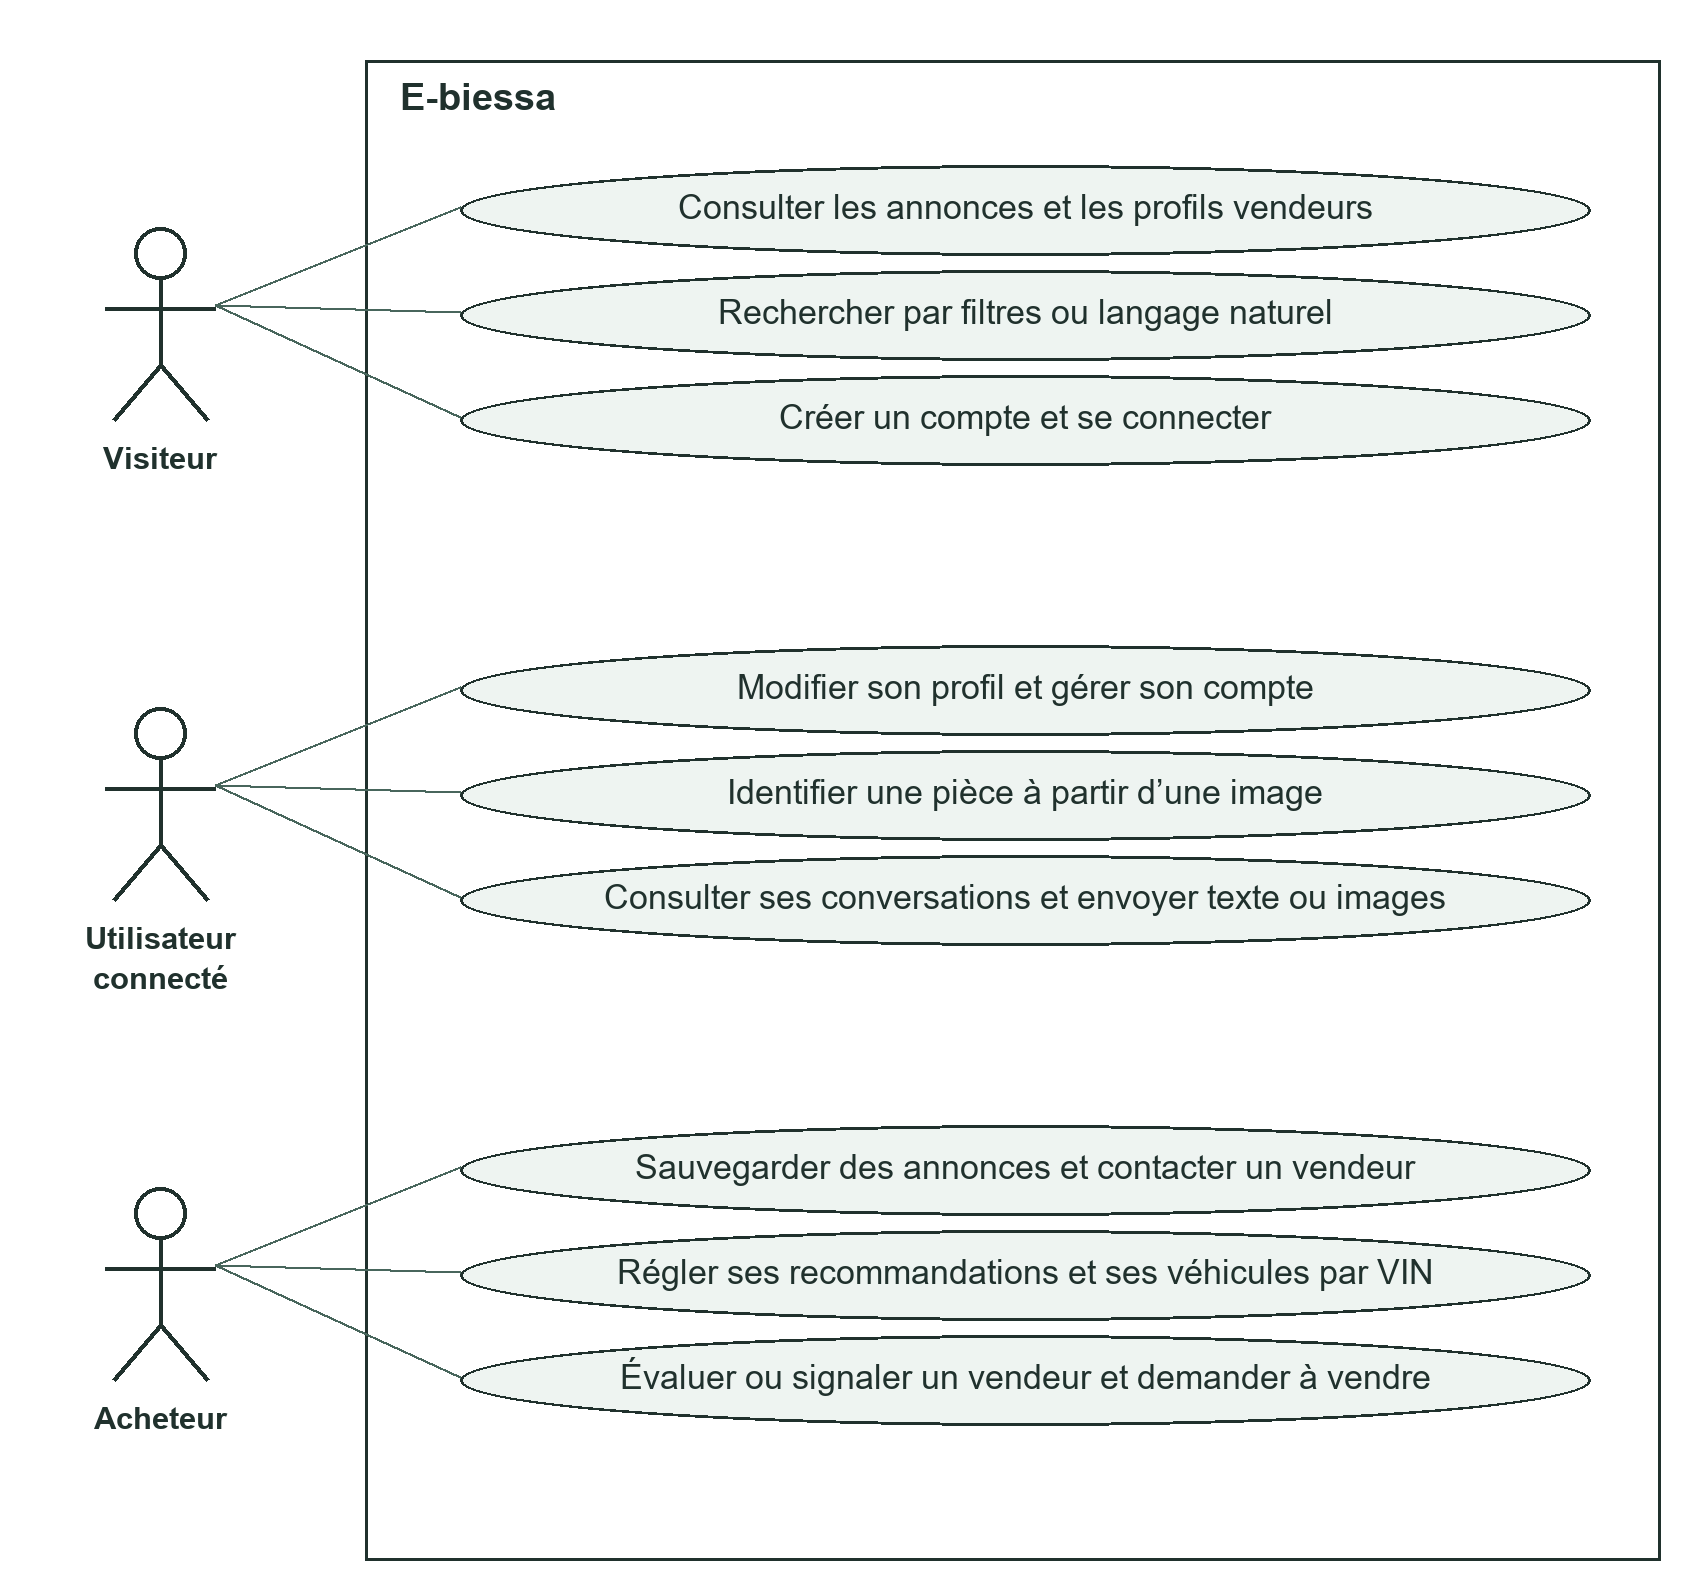
\includegraphics{images/figure-01.png}
\end{adjustbox}

\caption{Cas d'utilisation de consultation et d'achat}
\label{fig:report-1}
\end{figure}

Les fonctions d'utilisateur connecté sont communes aux rôles authentifiés. Les coordonnées, les avis et les recommandations personnalisées restent soumis aux contrôles du rôle acheteur. L'expression « achat » désigne ici la recherche et la mise en relation, sans paiement intégré.


\clearpage

\subsection{Publication et administration}

\begin{figure}[H]
\centering
\begin{adjustbox}{max width=\textwidth,max height=.64\textheight}
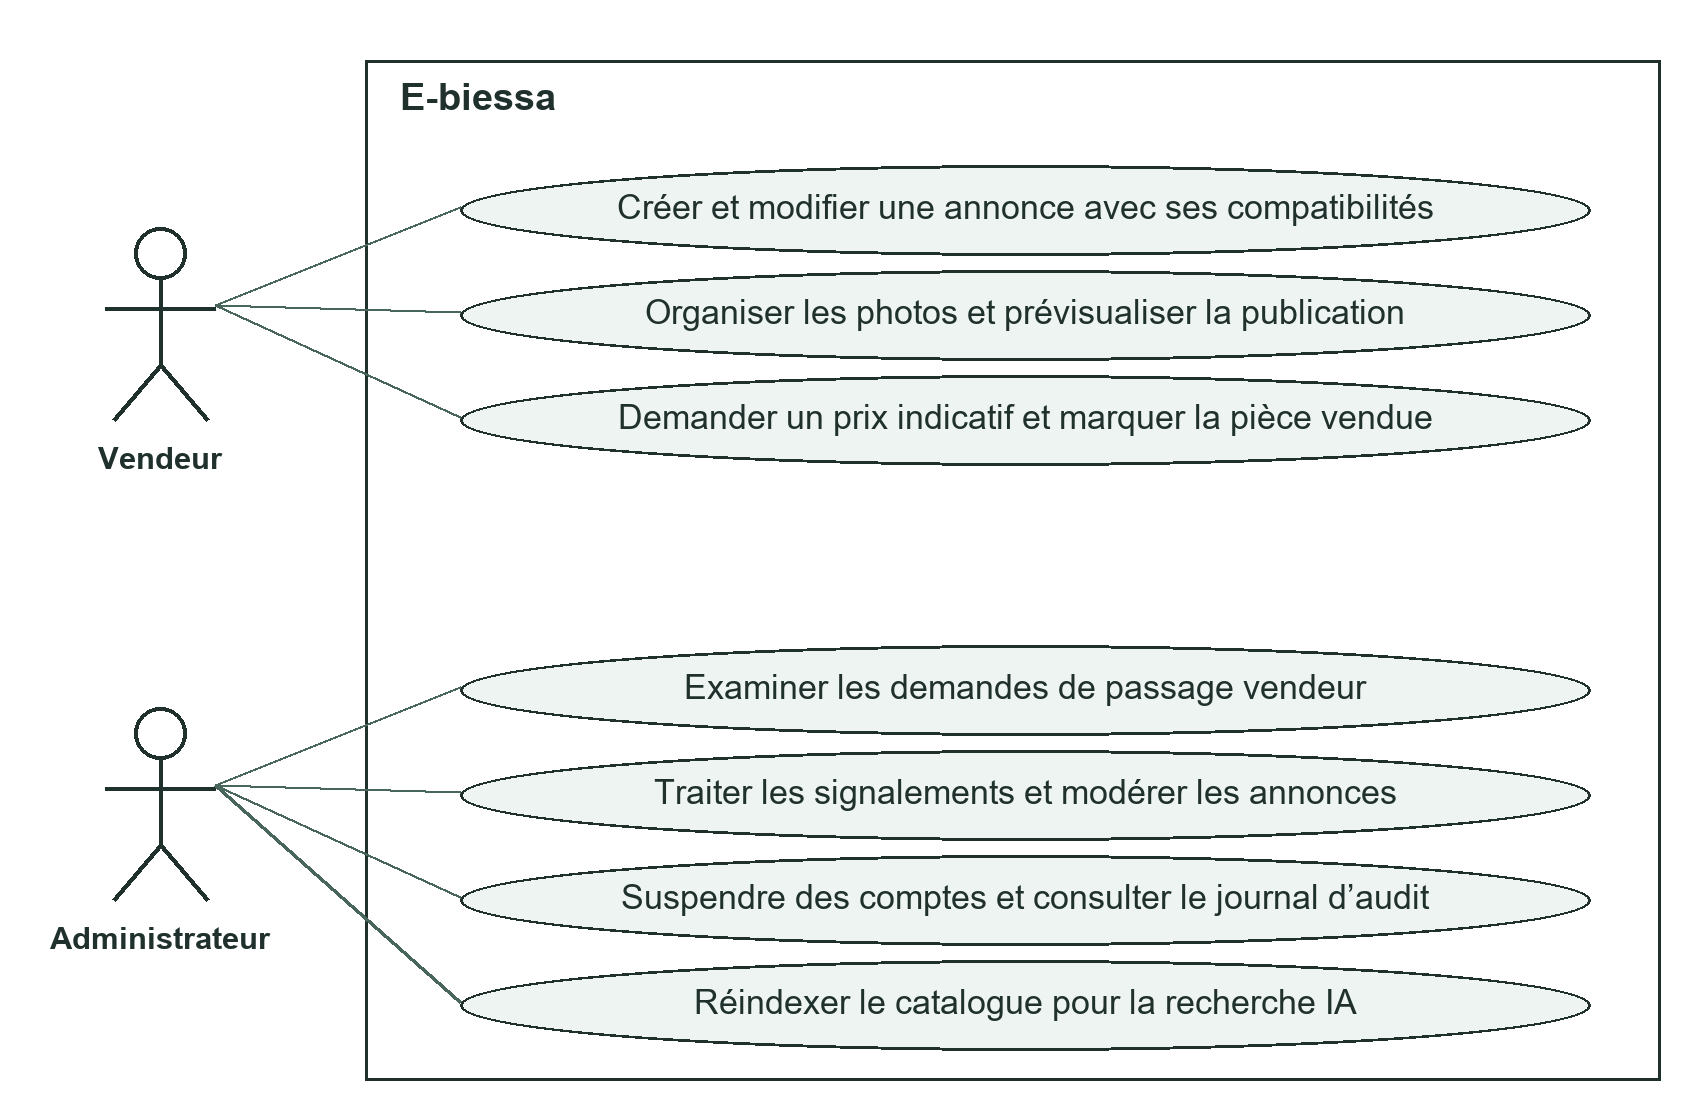
\includegraphics{images/figure-02.png}
\end{adjustbox}

\caption{Cas d'utilisation de vente et d'administration}
\label{fig:report-2}
\end{figure}

Le vendeur bénéficie des fonctions communes de compte et de messagerie. L'administrateur possède également les droits de gestion des annonces autorisés par le backend. La suspension et la résolution des signalements donnent lieu à des traces d'audit.


\subsection{Services externes et variantes}

{\small\singlespacing\arrayrulecolor{tableline}
\begin{longtable}{|>{\raggedright\arraybackslash}p{\dimexpr 0.350\textwidth-2\tabcolsep-2\arrayrulewidth\relax}|>{\raggedright\arraybackslash}p{\dimexpr 0.650\textwidth-2\tabcolsep-2\arrayrulewidth\relax}|}
\hline
\rowcolor{tablehead} \color{white}\bfseries Service externe & \color{white}\bfseries Interaction avec E-biessa \\ \hline
\endfirsthead
\rowcolor{tablehead} \color{white}\bfseries Service externe & \color{white}\bfseries Interaction avec E-biessa \\ \hline
\endhead
\hline\endfoot
Google, Facebook, Microsoft & Connexion OAuth quand le fournisseur est configuré. \\ \hline
\rowcolor{tablerow} SMTP et Twilio & Acheminement des codes de récupération selon la configuration. \\ \hline
CarQuery et NHTSA vPIC & Catalogue automobile et décodage VIN, avec limites de couverture. \\ \hline
\rowcolor{tablerow} Cloudinary & Stockage optionnel des images à la place du stockage local. \\ \hline
Service vocal du navigateur & Transcription soumise au support et aux permissions du navigateur. \\ \hline
\end{longtable}
}


Pour publier, le vendeur saisit les informations, consulte l'aperçu puis confirme l'envoi ; le serveur valide les champs et la propriété. Pour devenir vendeur, l'acheteur transmet sa demande et reste acheteur pendant l'examen. L'administrateur accepte ou refuse ; le rôle ne change qu'en cas d'acceptation. Pour contacter un vendeur, l'acheteur se connecte, ouvre une annonce active puis utilise les coordonnées autorisées ou crée une conversation.

\chapter{Conception}

La conception sépare les responsabilités transactionnelles, l'expérience utilisateur et le calcul d'intelligence artificielle afin de réduire le couplage et de garder les décisions critiques vérifiables.


\section{Choix d'architecture}

Le cahier des charges initial mettait l'accent sur FastAPI. Or, le socle transactionnel du projet a été stabilisé en Spring Boot. La décision finale conserve Spring comme coeur métier et exploite FastAPI comme microservice IA. Cette adaptation respecte les capacités demandées tout en évitant une réécriture risquée.


\textbf{Décision structurante}

Spring Boot est la frontière de sécurité et la source des réponses publiques. FastAPI ne reçoit que les documents nécessaires à l'indexation et renvoie des identifiants classés. Avant affichage, Spring recharge toujours les annonces depuis MySQL.


\begin{figure}[H]
\centering
\begin{adjustbox}{max width=\textwidth,max height=.64\textheight}
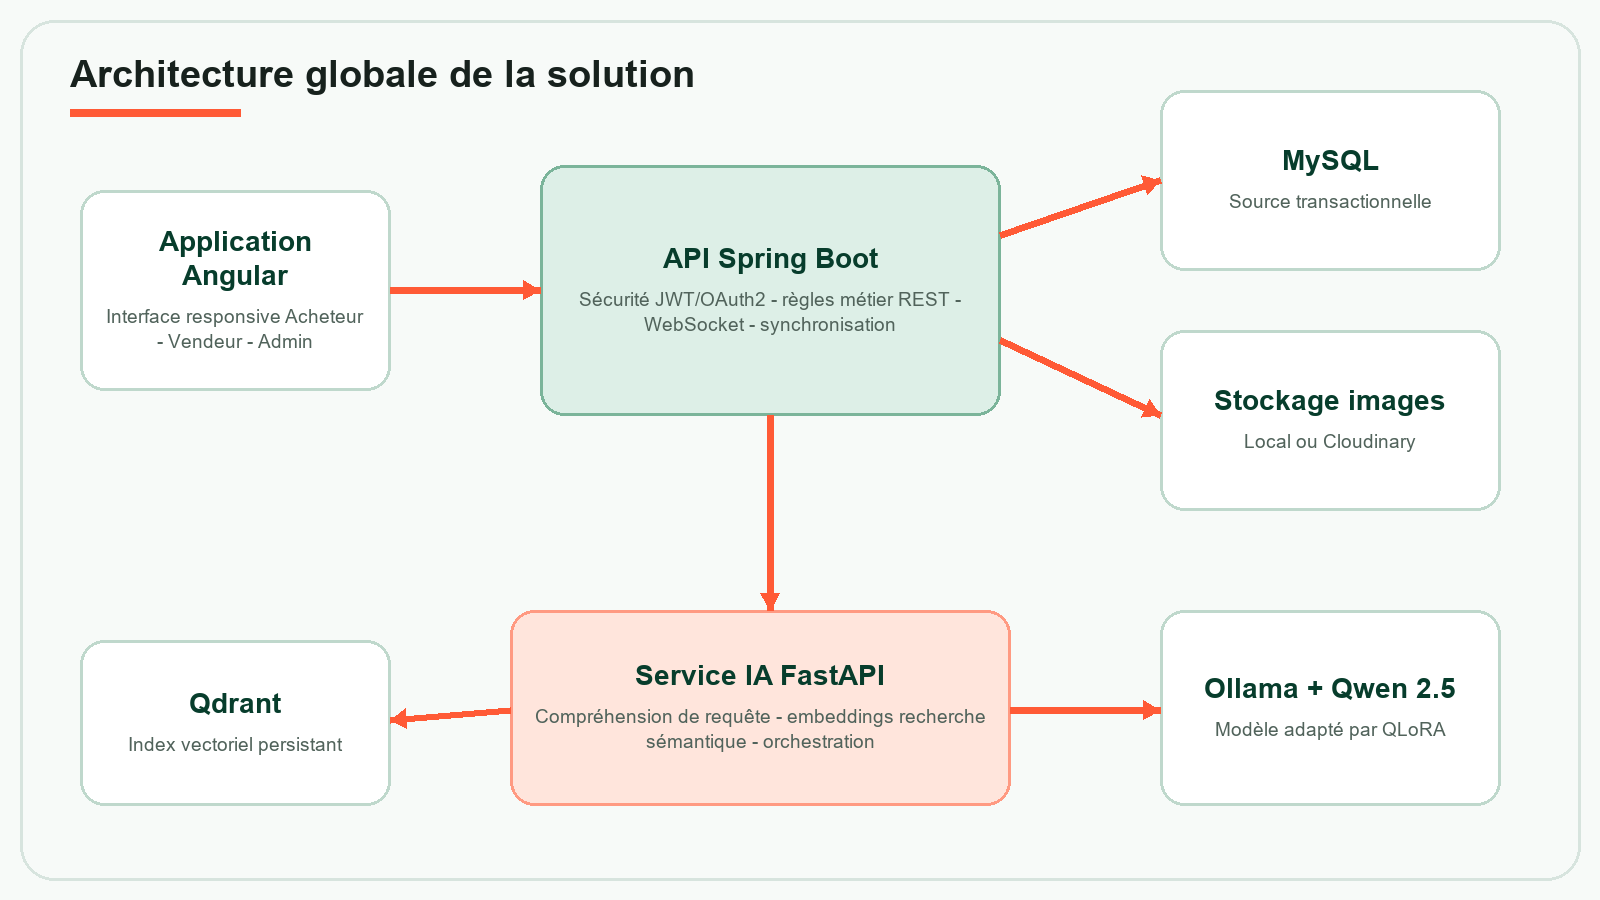
\includegraphics{images/figure-03.png}
\end{adjustbox}

\caption{Architecture globale de la solution}
\label{fig:report-3}
\end{figure}

\section{Architecture logique}

{\small\singlespacing\arrayrulecolor{tableline}
\begin{longtable}{|>{\raggedright\arraybackslash}p{\dimexpr 0.350\textwidth-2\tabcolsep-2\arrayrulewidth\relax}|>{\raggedright\arraybackslash}p{\dimexpr 0.650\textwidth-2\tabcolsep-2\arrayrulewidth\relax}|}
\hline
\rowcolor{tablehead} \color{white}\bfseries Couche & \color{white}\bfseries Responsabilité \\ \hline
\endfirsthead
\rowcolor{tablehead} \color{white}\bfseries Couche & \color{white}\bfseries Responsabilité \\ \hline
\endhead
\hline\endfoot
Présentation & Composants Angular, routes, formulaires, thèmes, retours d'erreur et accessibilité. \\ \hline
\rowcolor{tablerow} API & Contrôleurs REST, validation des DTO, sérialisation stable et contrats HTTP. \\ \hline
Métier & Services Spring portant autorisation, règles de cycle de vie, modération et classement. \\ \hline
\rowcolor{tablerow} Persistance & Dépôts JPA et modèle relationnel MySQL ; Qdrant pour les vecteurs reconstruisibles. \\ \hline
IA & Embeddings, extraction de contraintes, récupération, agents spécialisés et explications. \\ \hline
\rowcolor{tablerow} Infrastructure & Stockage d'images, courriel/SMS optionnels, OAuth et catalogue véhicule externe avec repli local. \\ \hline
\end{longtable}
}


\section{Modèle de données}

L'entité Utilisateur centralise l'identité et le rôle. Une annonce appartient à un vendeur, à une catégorie et à une collection de véhicules compatibles. Les images conservent un ordre et une image principale. Les conversations relient un acheteur, un vendeur et l'annonce d'origine. Les signaux d'activité restent séparés des messages et des coordonnées afin de limiter les données utilisées pour la personnalisation.


Les quatre vues suivantes forment le diagramme de classes du domaine persistant. Les noms correspondent aux entités Java ; les attributs sont sélectionnés pour la lisibilité. Les associations portent leurs multiplicités. Les rôles BUYER, SELLER et ADMIN sont les valeurs de UserRole, et non des sous-classes de User. Les méthodes métier appartiennent aux services, non aux entités représentées.


\clearpage

\subsection{Catalogue et favoris}

\begin{figure}[H]
\centering
\begin{adjustbox}{max width=\textwidth,max height=.64\textheight}
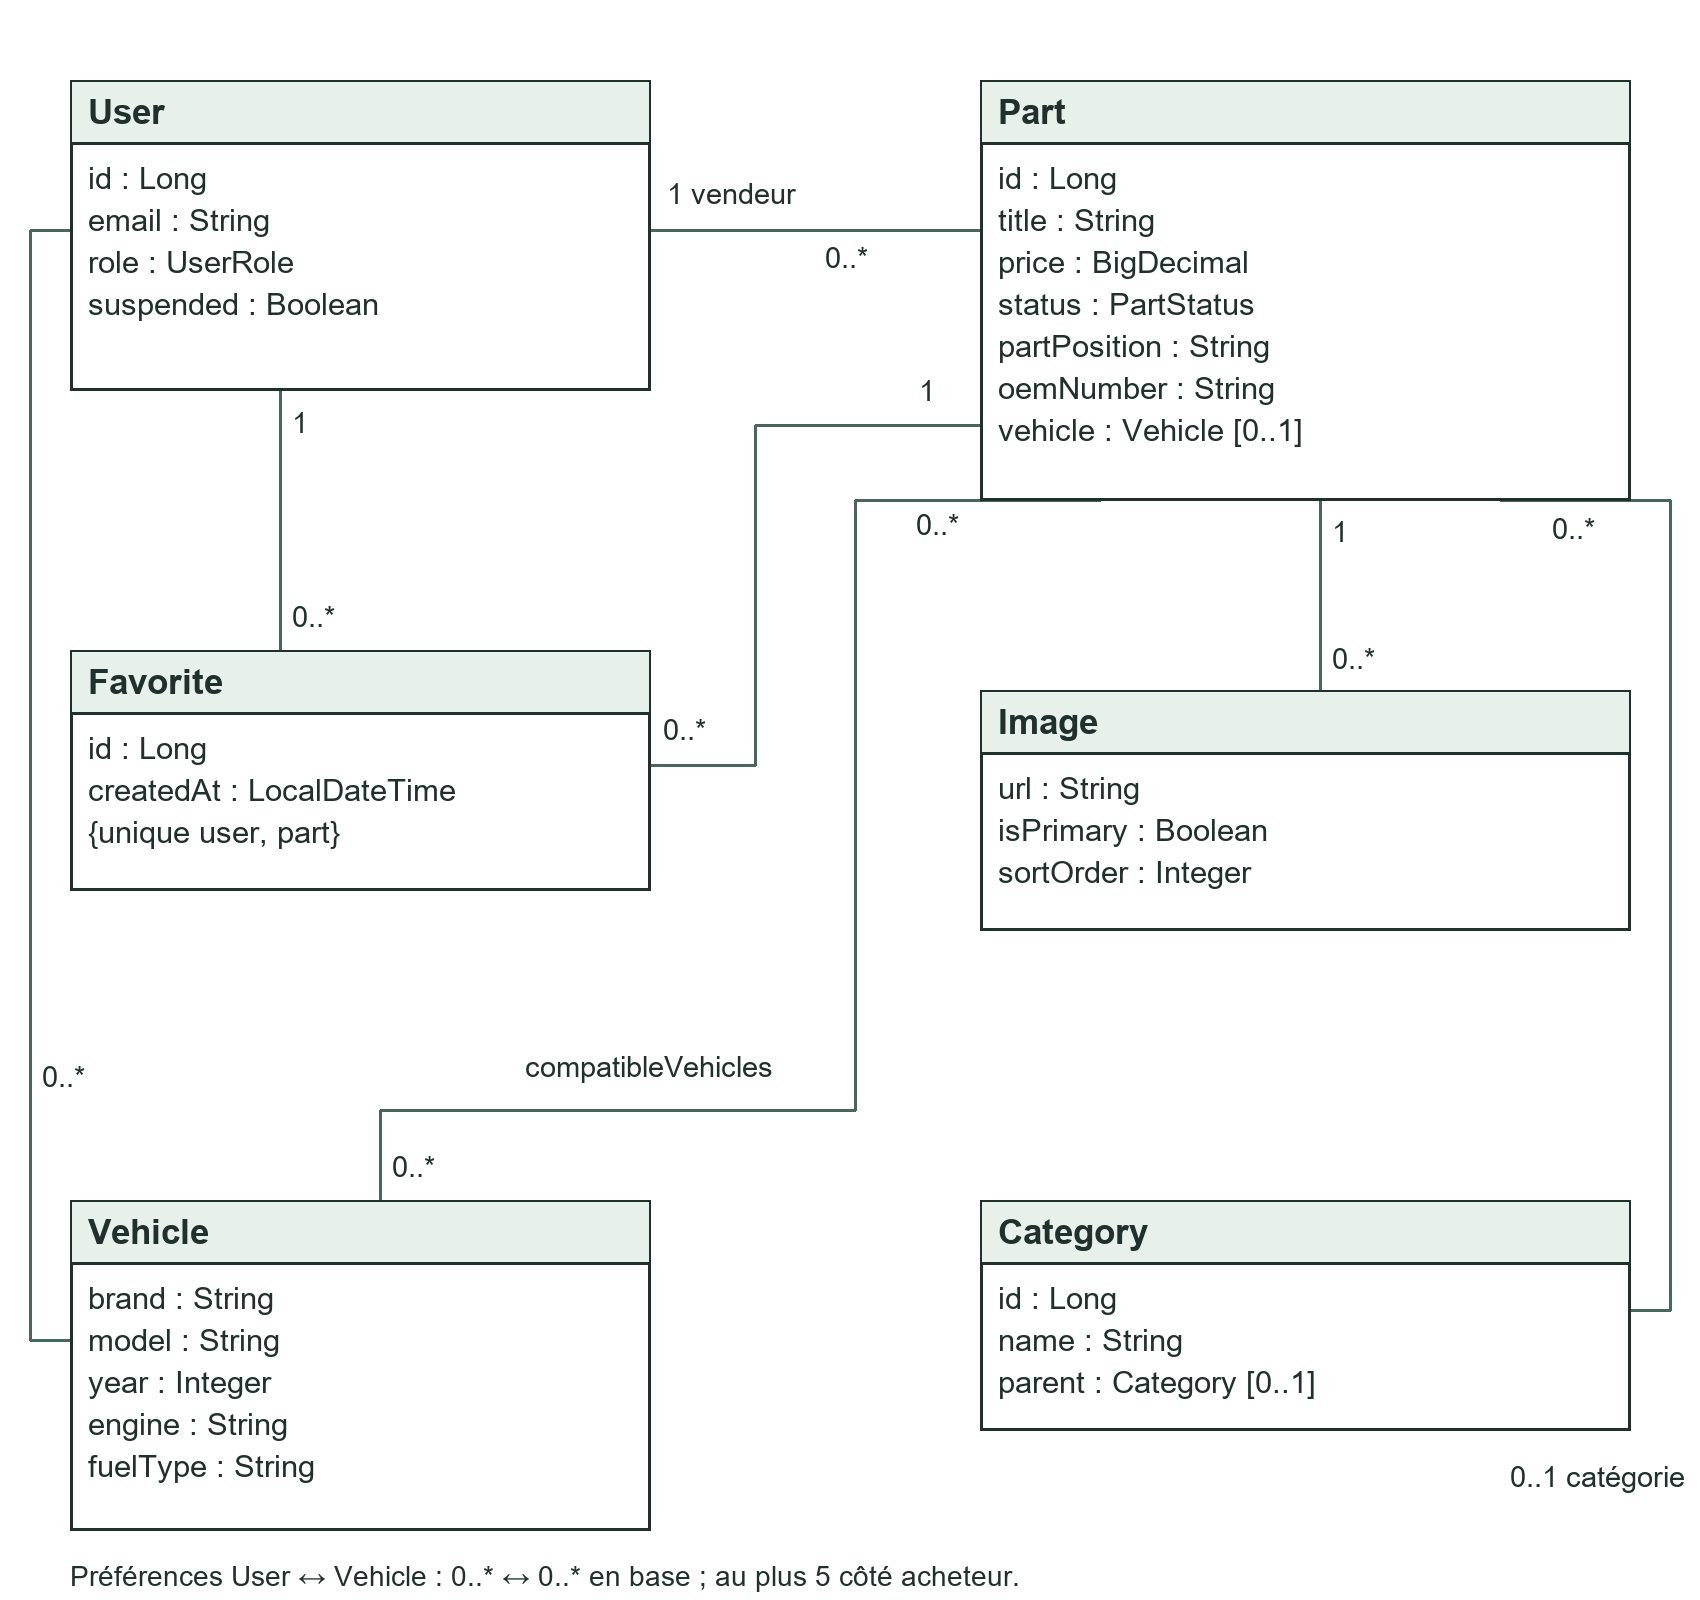
\includegraphics{images/figure-04.png}
\end{adjustbox}

\caption{Classes du catalogue et des favoris}
\label{fig:report-4}
\end{figure}

Part et Vehicle sont reliés par part\_compatible\_vehicles. Le lien historique Part.vehicle est maintenu séparément pour la compatibilité des données existantes. Category possède un parent facultatif et zéro à plusieurs sous-catégories. Les restrictions moteur et carburant de Part complètent les caractéristiques des véhicules ; elles ne constituent pas une entité de compatibilité distincte.


\clearpage

\subsection{Conversations et réputation}

\begin{figure}[H]
\centering
\begin{adjustbox}{max width=\textwidth,max height=.64\textheight}
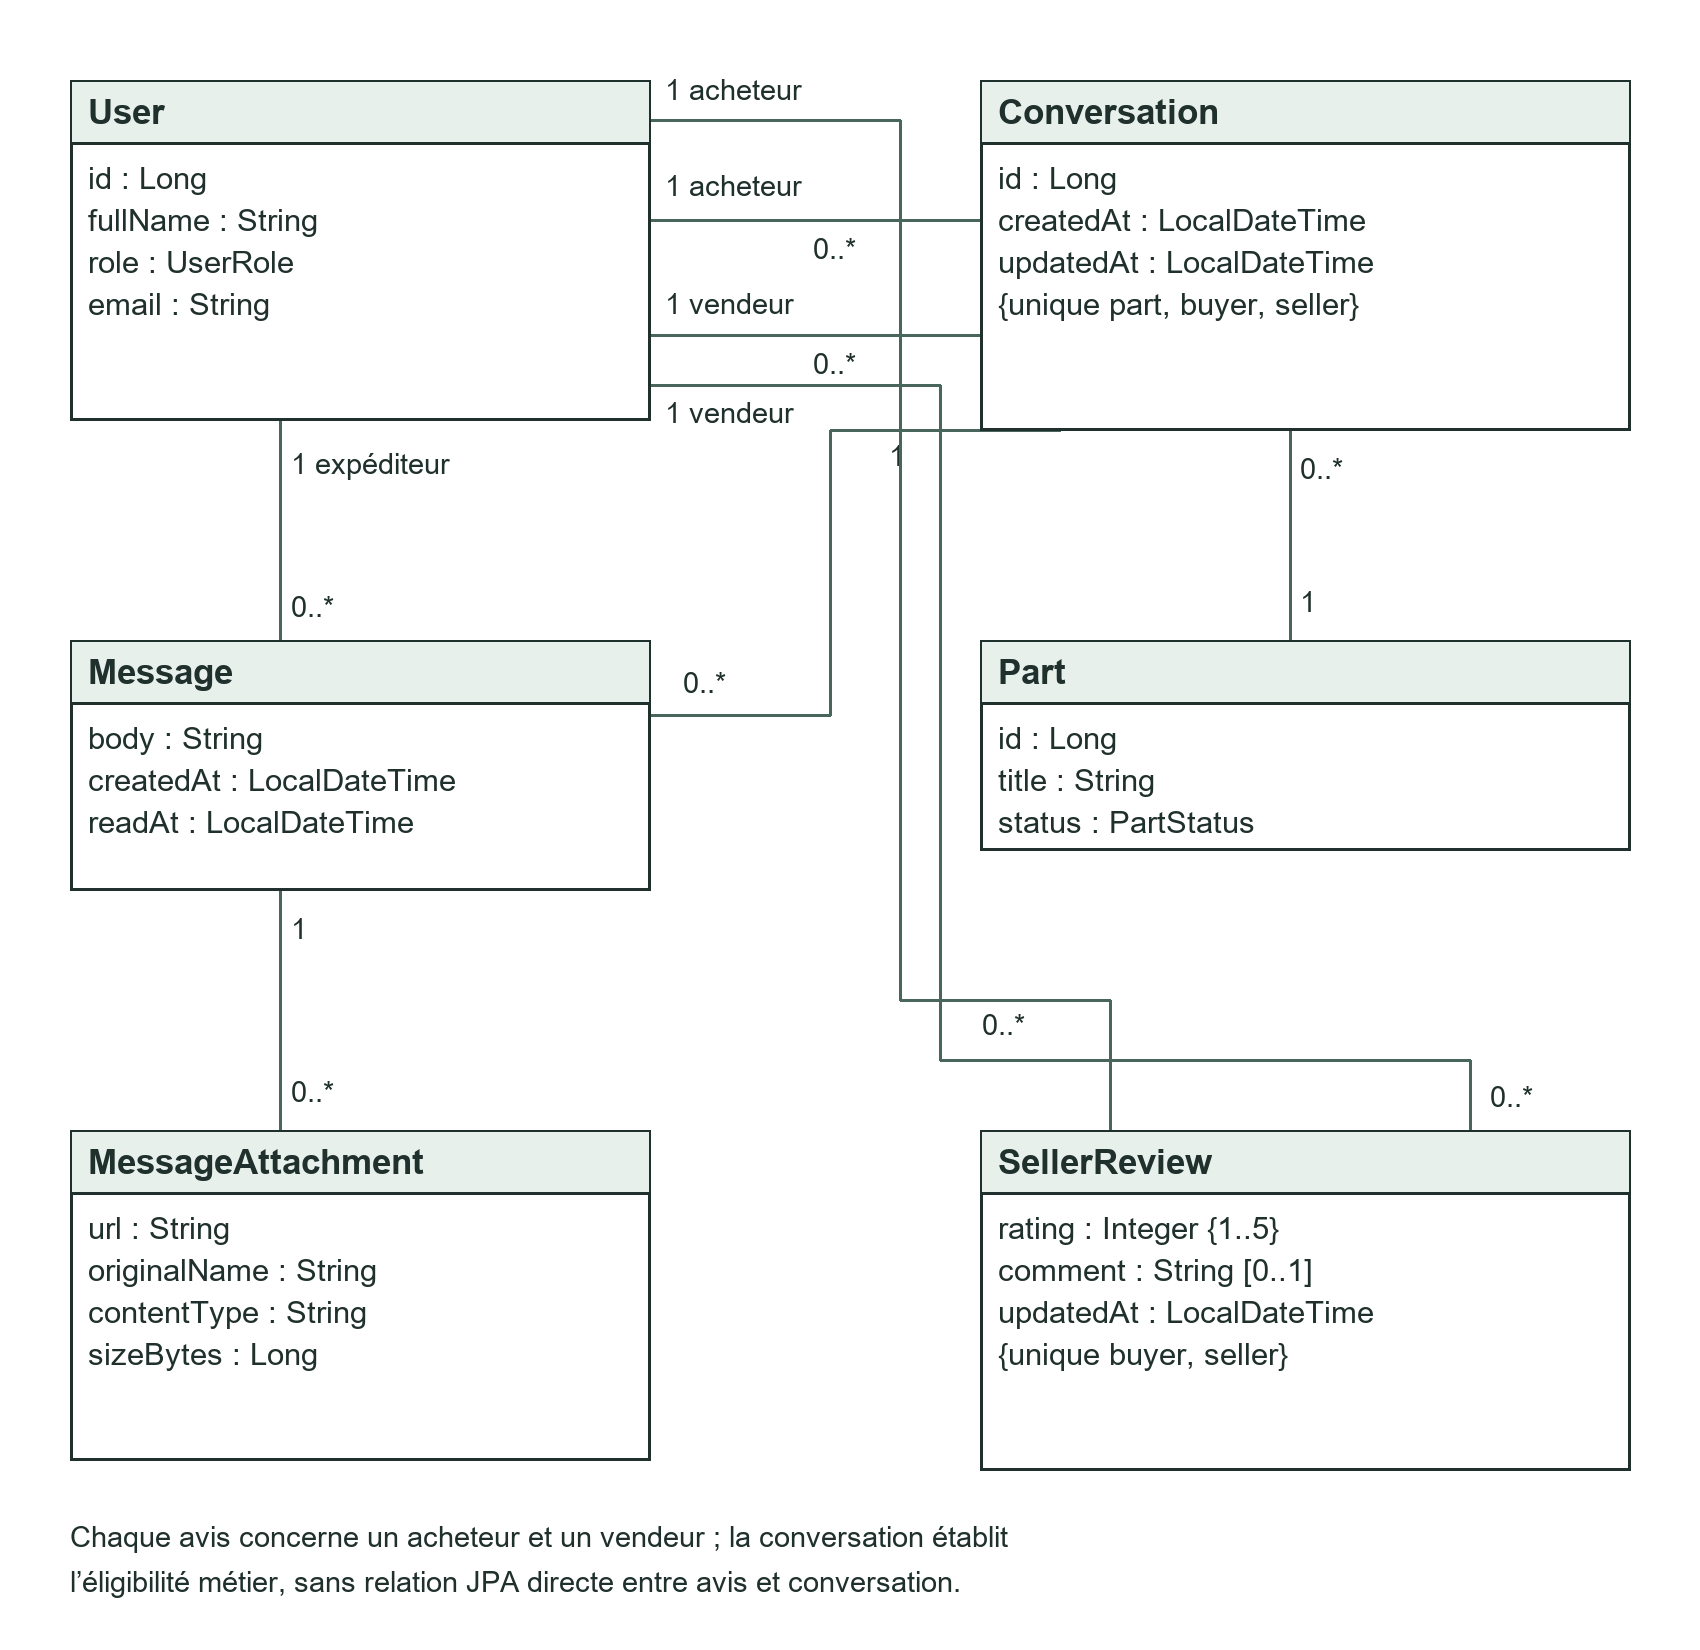
\includegraphics{images/figure-05.png}
\end{adjustbox}

\caption{Classes de communication et de réputation}
\label{fig:report-5}
\end{figure}

Une conversation relie exactement une annonce, un acheteur et un vendeur. Elle contient zéro à plusieurs messages ; chaque message a un seul expéditeur et zéro à plusieurs pièces jointes. Les avis référencent directement les deux utilisateurs. Les autorisations vérifient que l'expéditeur appartient à la conversation.


\clearpage

\subsection{Identité et personnalisation}

\begin{figure}[H]
\centering
\begin{adjustbox}{max width=\textwidth,max height=.64\textheight}
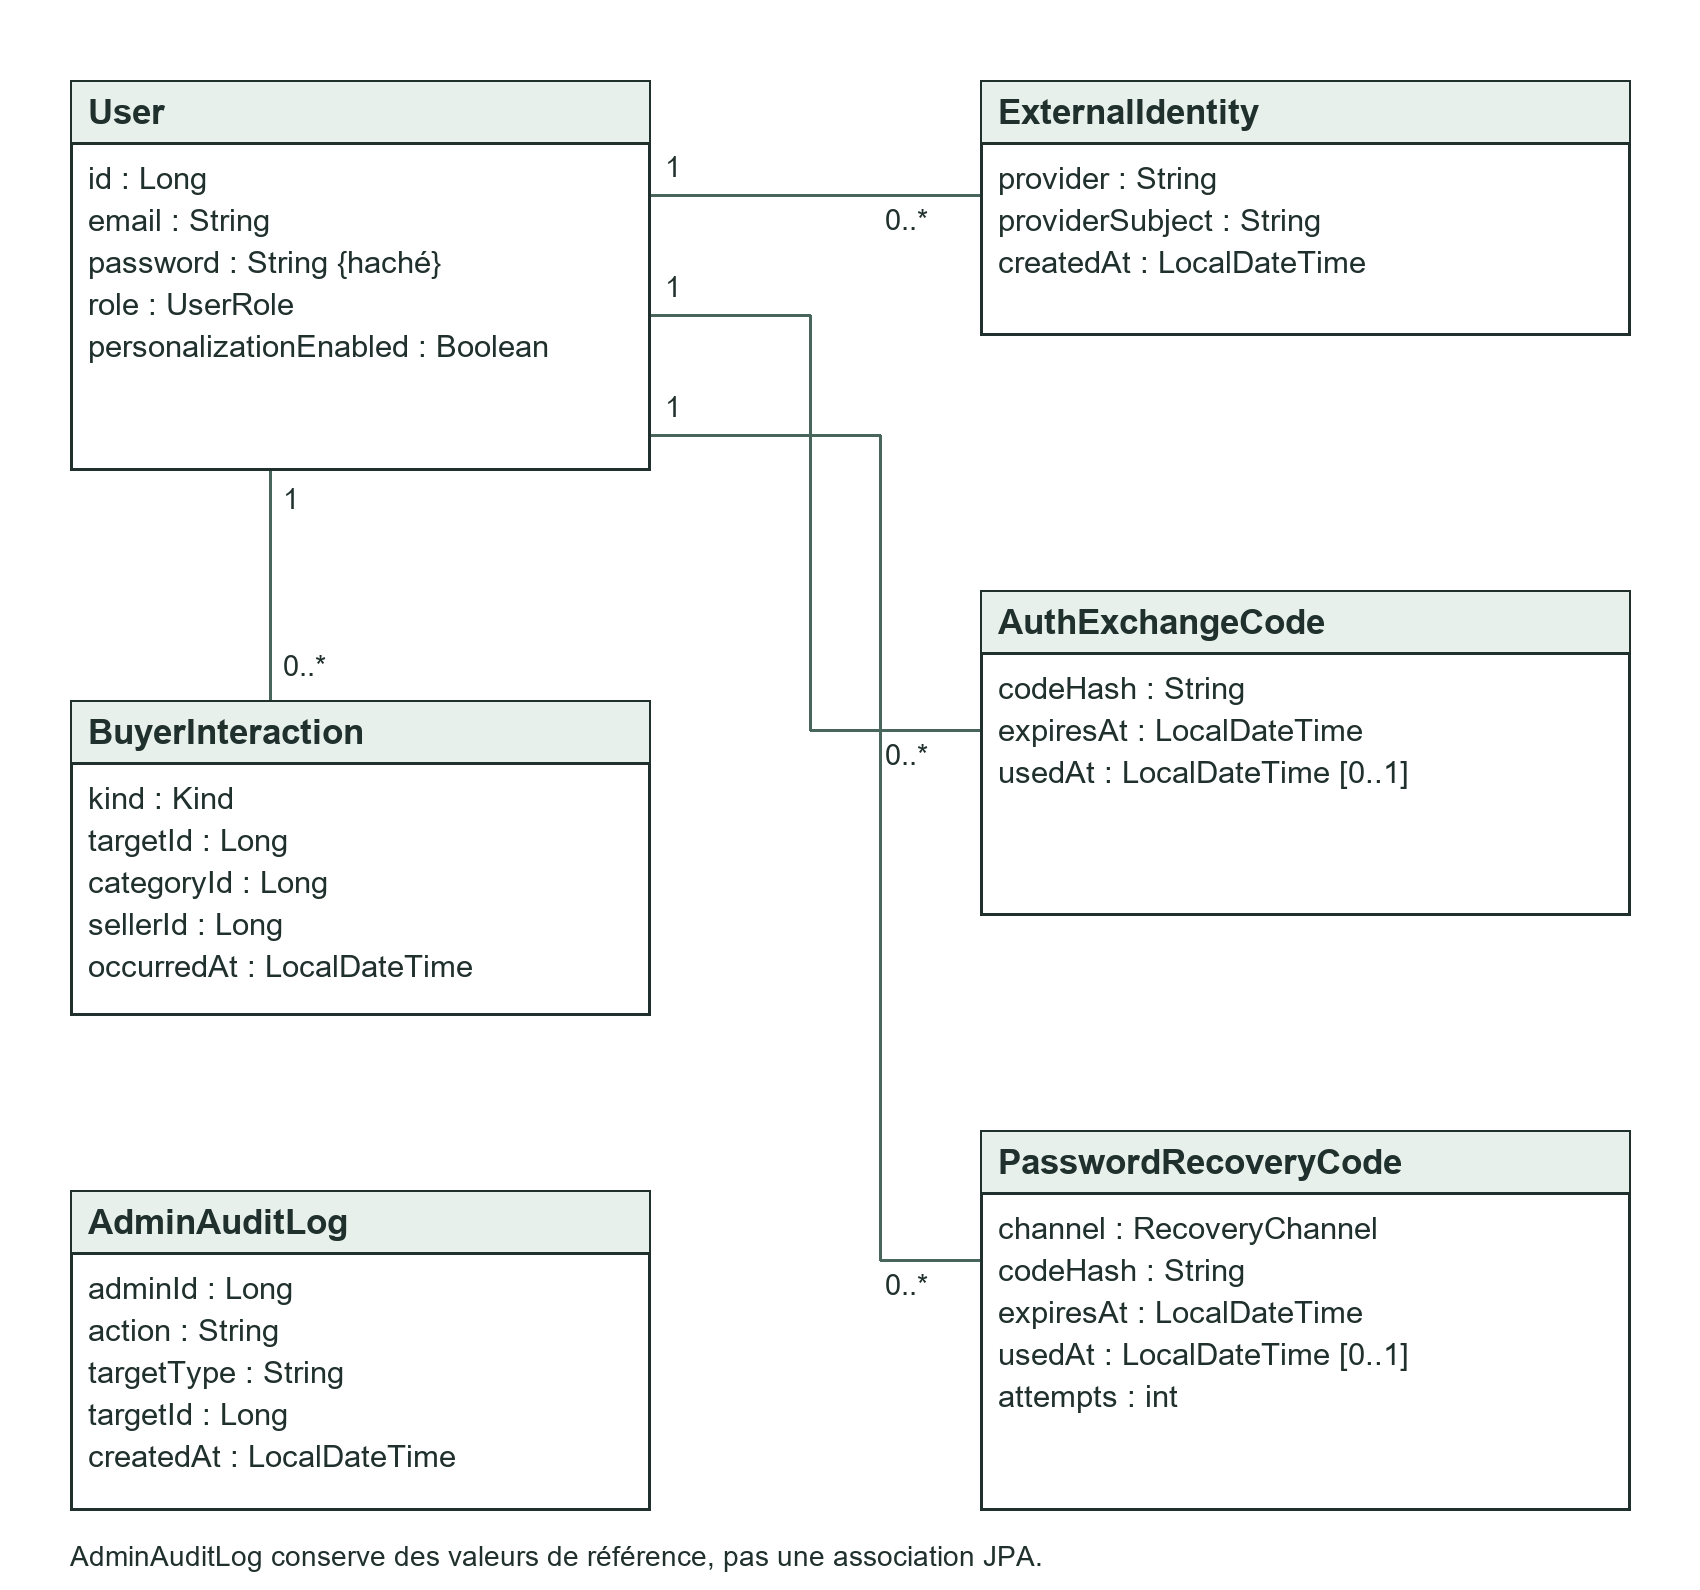
\includegraphics{images/figure-06.png}
\end{adjustbox}

\caption{Classes d'identité et de personnalisation}
\label{fig:report-6}
\end{figure}

Les codes temporaires sont associés à un utilisateur et stockés sous forme de condensat. BuyerInteraction contient des références numériques de contexte et n'établit pas de relations JPA vers Part ou Category. AdminAuditLog conserve un instantané d'identifiants et de libellés pour préserver la trace d'une action.


\clearpage

\subsection{Signalements et validation des vendeurs}

\begin{figure}[H]
\centering
\begin{adjustbox}{max width=\textwidth,max height=.64\textheight}
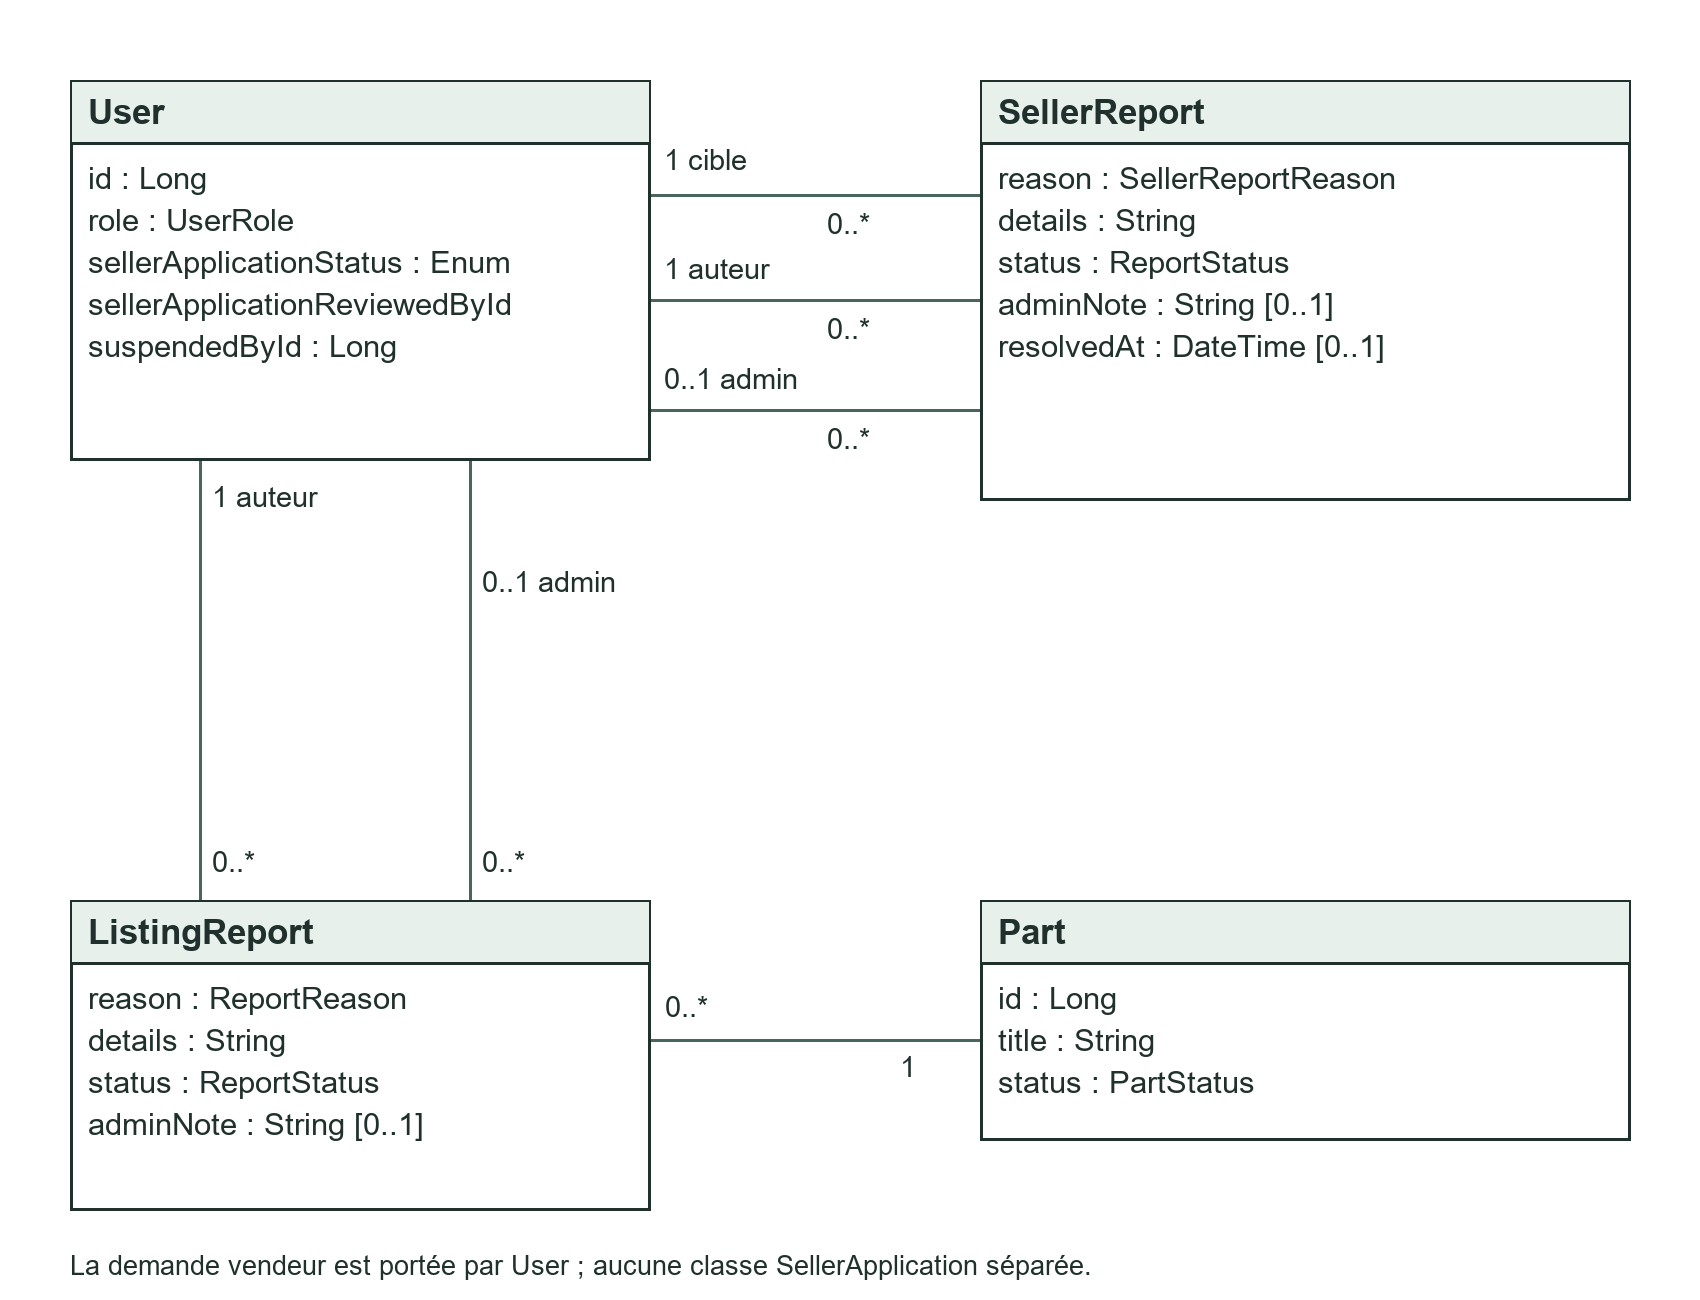
\includegraphics{images/figure-07.png}
\end{adjustbox}

\caption{Classes de modération}
\label{fig:report-7}
\end{figure}

SellerReport et ListingReport distinguent l'auteur, la cible et l'administrateur résolveur facultatif. La demande de passage vendeur est représentée par des champs de User, dont le statut et les dates de traitement. L'acceptation change le rôle ; le dépôt d'une demande ne crée pas automatiquement un vendeur.


Les structures de recherche, VIN, prix et vision sont des DTO ou des résultats temporaires de services. Elles ne créent pas de tables JPA supplémentaires. L'index Qdrant est reconstructible à partir de MySQL et n'est pas un second référentiel transactionnel. Les champs d'identité sont réservés aux DTO autorisés et ne sont pas tous exposés dans les profils publics.


\clearpage

\section{Conception de la recherche intelligente}

Une annonce active est transformée en document textuel normalisé contenant titre, description, catégorie, références et compatibilités. FastEmbed calcule son vecteur multilingue, stocké dans la collection Qdrant. Lors d'une requête, Qwen extrait un objet JSON. Le système fusionne cette sortie avec les contraintes lexicales et les filtres explicites, puis récupère des candidats sémantiques.


Le classement final applique un seuil minimal et vérifie les contraintes sur une même ligne de compatibilité. Les raisons visibles - par exemple « compatible Golf », « diesel », « position arrière » ou « système de freinage » - proviennent des champs réellement associés à l'annonce. La réponse est construite par Spring à partir des DTO actifs, ce qui empêche une prose générée ou un identifiant périmé de devenir une recommandation publique.


\begin{figure}[H]
\centering
\begin{adjustbox}{max width=\textwidth,max height=.64\textheight}
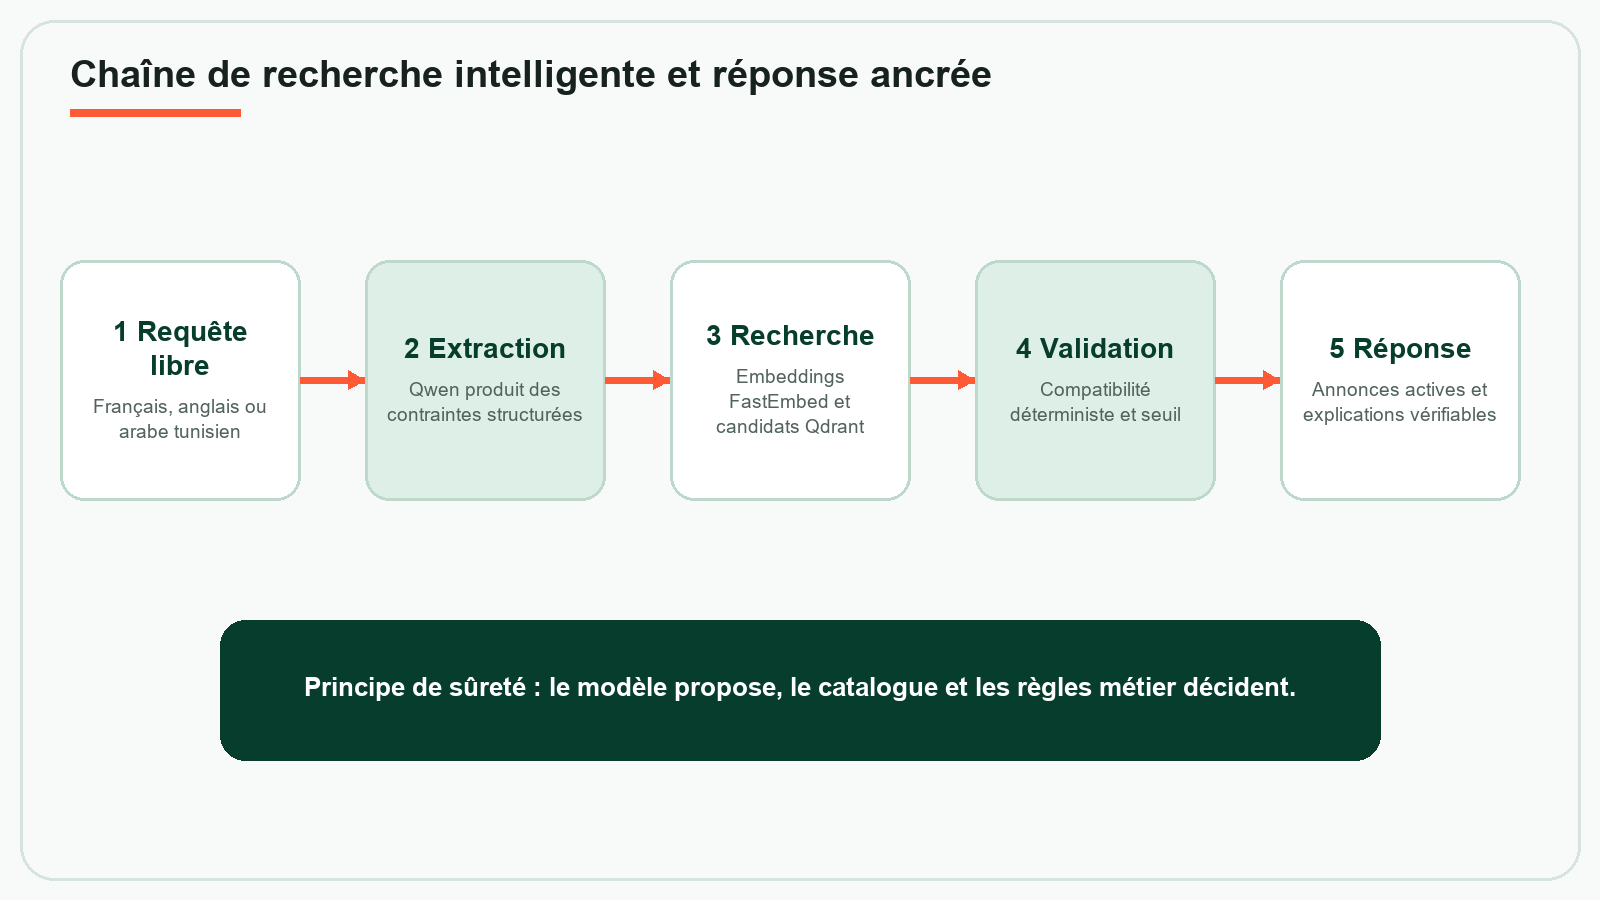
\includegraphics{images/figure-08.png}
\end{adjustbox}

\caption{Chaîne de recherche intelligente et réponse ancrée}
\label{fig:report-8}
\end{figure}

\section{Orchestration agentique finale}

La couche LangChain encapsule trois outils StructuredTool : search\_agent, compatibility\_agent et recommendation\_agent. Le routage est déterministe : la recherche s'exécute d'abord, la vérification des contraintes suit si nécessaire, puis les candidats personnalisés fournis par Spring peuvent être intégrés selon l'intention détectée. Il ne s'agit pas d'agents autonomes qui planifient librement des actions. Aucun outil ne crée, ne modifie ou ne supprime une donnée métier.


{\small\singlespacing\arrayrulecolor{tableline}
\begin{longtable}{|>{\raggedright\arraybackslash}p{\dimexpr 0.230\textwidth-2\tabcolsep-2\arrayrulewidth\relax}|>{\raggedright\arraybackslash}p{\dimexpr 0.250\textwidth-2\tabcolsep-2\arrayrulewidth\relax}|>{\raggedright\arraybackslash}p{\dimexpr 0.260\textwidth-2\tabcolsep-2\arrayrulewidth\relax}|>{\raggedright\arraybackslash}p{\dimexpr 0.260\textwidth-2\tabcolsep-2\arrayrulewidth\relax}|}
\hline
\rowcolor{tablehead} \color{white}\bfseries Agent & \color{white}\bfseries Entrées & \color{white}\bfseries Sortie autorisée & \color{white}\bfseries Garde-fou \\ \hline
\endfirsthead
\rowcolor{tablehead} \color{white}\bfseries Agent & \color{white}\bfseries Entrées & \color{white}\bfseries Sortie autorisée & \color{white}\bfseries Garde-fou \\ \hline
\endhead
\hline\endfoot
Recherche & Texte et filtres & Identifiants candidats & Limite et seuil de pertinence \\ \hline
\rowcolor{tablerow} Compatibilité & Contraintes et fiche annonce & Candidats conservés après revalidation & Règles catalogue prioritaires \\ \hline
Recommandation & Candidats assainis fournis par Spring et limite & Suggestions et raisons & Pas de données inter-utilisateurs \\ \hline
\rowcolor{tablerow} Orchestrateur & Intention utilisateur & Plan court et réponse structurée & Lecture seule, délai et nombre d'appels bornés \\ \hline
\end{longtable}
}


\section{Sécurité}

\begin{itemize}
\item identité extraite du contexte JWT, jamais d'un identifiant fourni librement par le client ;

\item autorisation par rôle au niveau des routes et réévaluation de la propriété dans les services ;

\item codes OAuth courts, à usage unique, sans JWT dans l'URL de redirection ;

\item codes de récupération expirables, nombre d'essais limité et réponses non révélatrices ;

\item jetons WebSocket courts et à usage unique pour éviter de transmettre le JWT dans une chaîne de requête ;

\item signature réelle des fichiers image contrôlée en plus du type MIME déclaré ;

\item jeton interne partagé entre Spring et FastAPI pour les opérations d'indexation ;

\item limitation de débit, concurrence bornée, cache court et délai maximum sur l'endpoint IA public ;

\item secrets chargés depuis l'environnement et exclus de Git.
\end{itemize}

\clearpage

\section{Conception de la messagerie}

La messagerie suit un modèle conversationnel unique par contexte d'annonce. Le chargement initial place la vue sur le dernier message, tandis que le contenu reste dans une zone de hauteur limitée et défilable. Les événements WebSocket mettent à jour l'interface sans recharger la page. Les images jointes sont stockées via le même contrat que les images d'annonces, avec des limites dédiées.


\begin{figure}[H]
\centering
\begin{adjustbox}{max width=\textwidth,max height=.64\textheight}
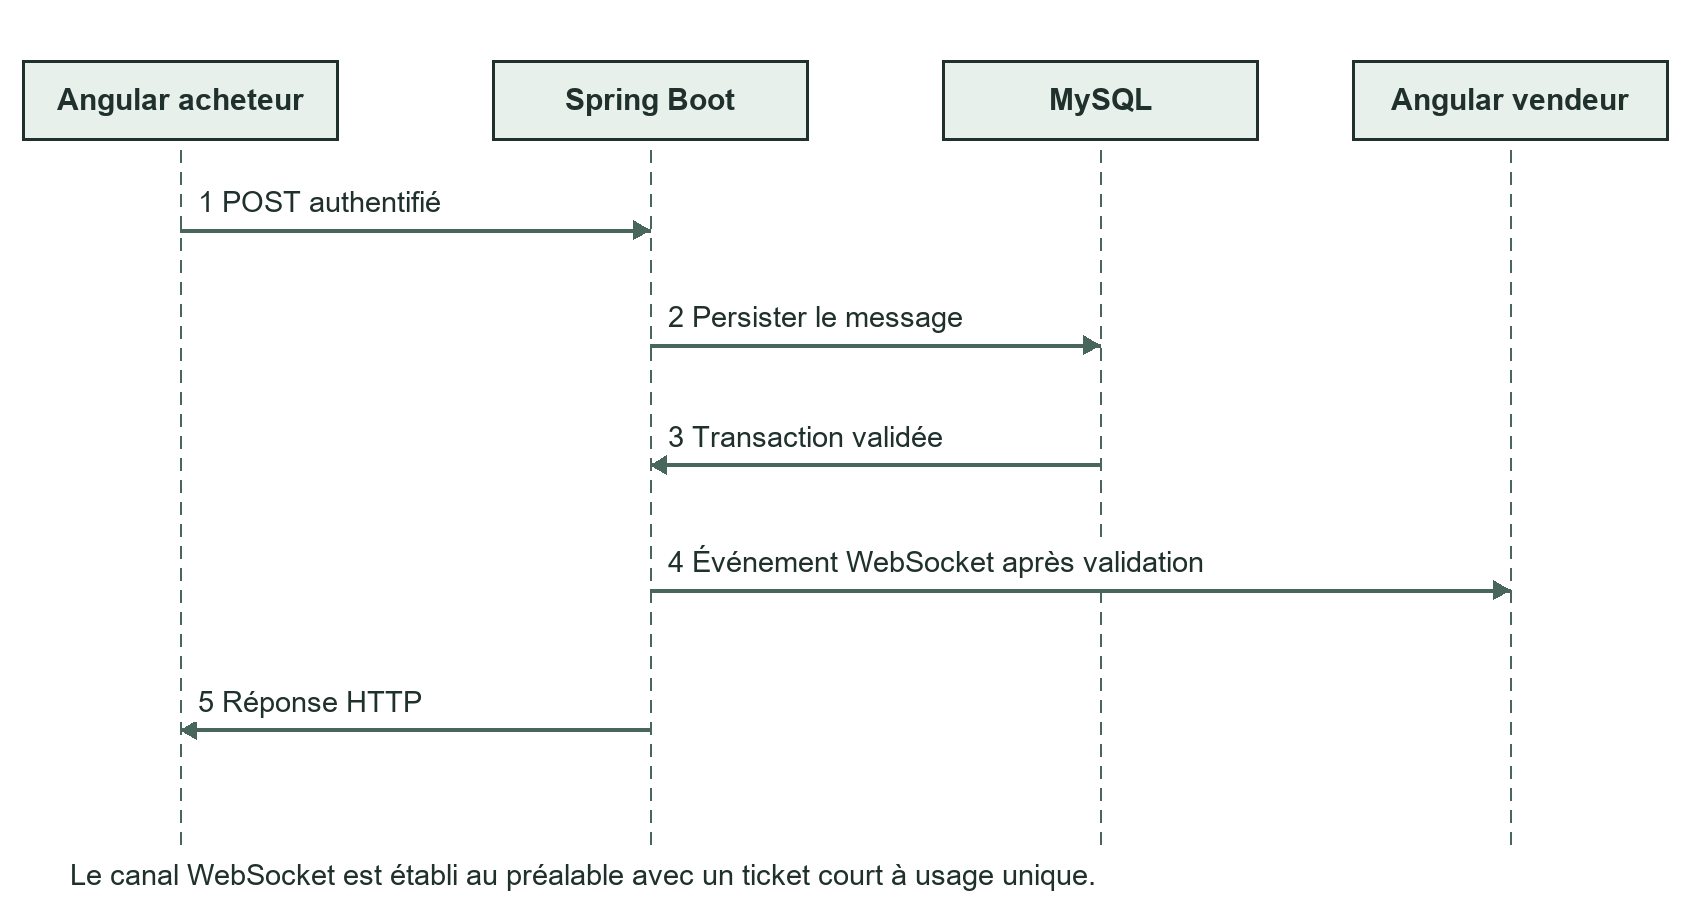
\includegraphics{images/figure-09.png}
\end{adjustbox}

\caption{Séquence simplifiée de la messagerie instantanée}
\label{fig:report-9}
\end{figure}

\clearpage

\section{Conception de la recommandation}

Le moteur combine compatibilité déclarée, catégories sauvegardées, vendeurs contactés, popularité et récence. Les préférences véhicule agissent comme contrainte forte. Les interactions comportementales sont dédupliquées, limitées à 200 enregistrements, pondérées avec une demi-vie de trente jours et ignorées après quatre-vingt-dix jours. Le score reste un rang interne et n'est jamais présenté comme un pourcentage de compatibilité.


\begin{figure}[H]
\centering
\begin{adjustbox}{max width=\textwidth,max height=.64\textheight}
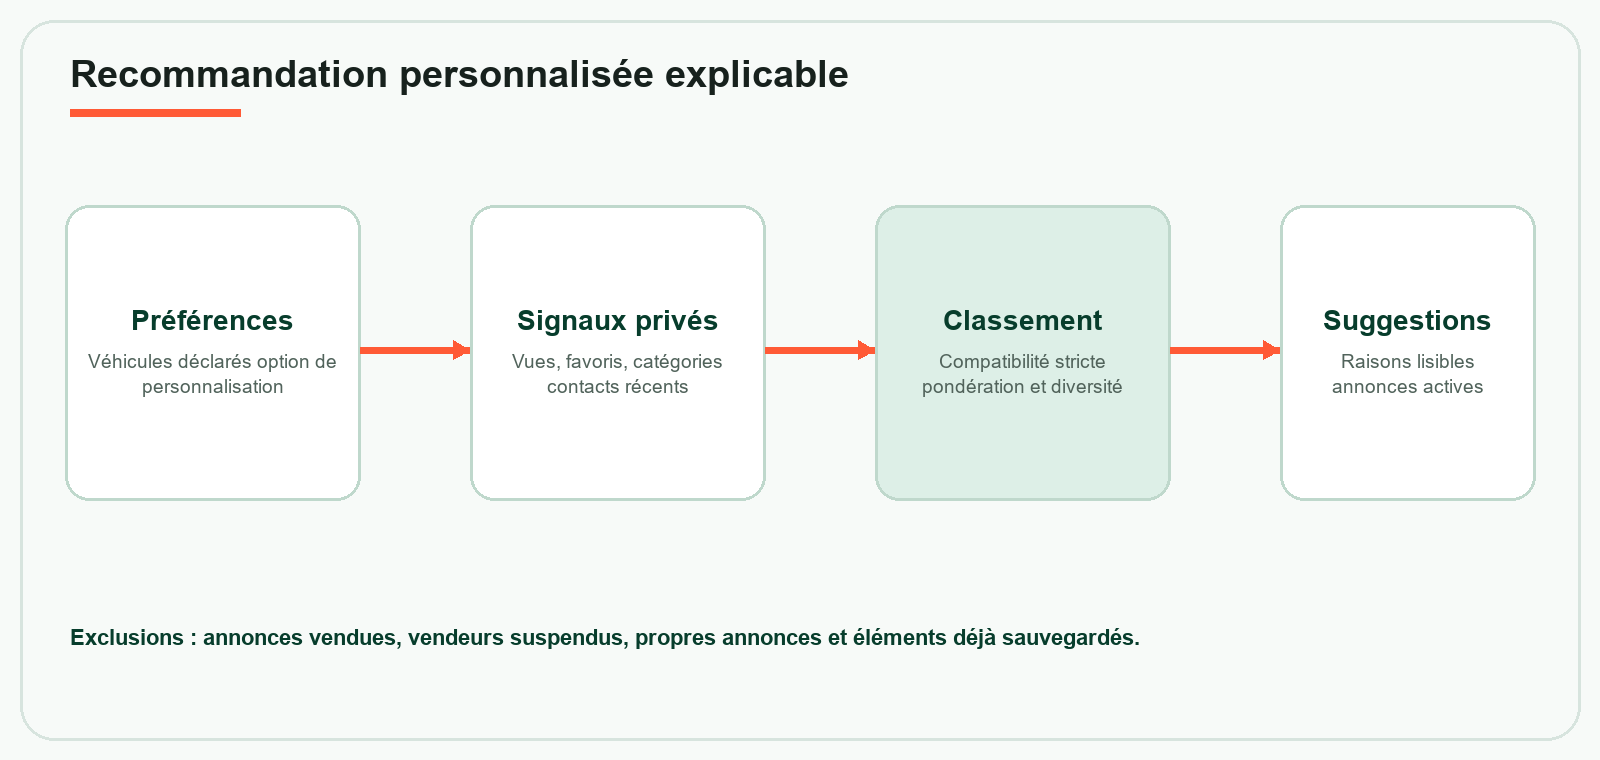
\includegraphics{images/figure-10.png}
\end{adjustbox}

\caption{Recommandation personnalisée explicable}
\label{fig:report-10}
\end{figure}

\chapter{Réalisation}

Cette partie présente l'environnement technique, les principaux modules développés et l'intégration finale des services.


\section{Environnement de travail}

{\small\singlespacing\arrayrulecolor{tableline}
\begin{longtable}{|>{\raggedright\arraybackslash}p{\dimexpr 0.240\textwidth-2\tabcolsep-2\arrayrulewidth\relax}|>{\raggedright\arraybackslash}p{\dimexpr 0.320\textwidth-2\tabcolsep-2\arrayrulewidth\relax}|>{\raggedright\arraybackslash}p{\dimexpr 0.440\textwidth-2\tabcolsep-2\arrayrulewidth\relax}|}
\hline
\rowcolor{tablehead} \color{white}\bfseries Élément & \color{white}\bfseries Choix final & \color{white}\bfseries Rôle \\ \hline
\endfirsthead
\rowcolor{tablehead} \color{white}\bfseries Élément & \color{white}\bfseries Choix final & \color{white}\bfseries Rôle \\ \hline
\endhead
\hline\endfoot
Langage backend & Java 21 & API transactionnelle et règles métier \\ \hline
\rowcolor{tablerow} Framework backend & Spring Boot 3.2.8 & Web, sécurité, validation, JPA et WebSocket \\ \hline
Frontend & Angular 21, TypeScript 5.9 & SPA responsive et formulaires réactifs \\ \hline
\rowcolor{tablerow} Service IA & Python 3.12, FastAPI & Recherche sémantique et orchestration \\ \hline
Données & MySQL, Qdrant & Source de vérité relationnelle et index vectoriel \\ \hline
\rowcolor{tablerow} Modèle & Qwen 2.5 7B Instruct & Extraction multilingue de contraintes \\ \hline
Adaptation & Unsloth QLoRA & Entraînement local quantifié \\ \hline
\rowcolor{tablerow} Exécution LLM & Ollama & Inférence locale sur GPU \\ \hline
Tests & JUnit, Vitest, Pytest, Playwright & Validation multi-couche \\ \hline
\rowcolor{tablerow} Versionnement & Git et GitHub & Historique, partage et sauvegarde du code \\ \hline
\end{longtable}
}


\section{Backend Spring Boot}

Le backend applique une organisation par contrôleurs, services, dépôts, entités et DTO. Les contrôleurs exposent les contrats HTTP et délèguent les décisions aux services. Les DTO empêchent la sérialisation directe des entités JPA et stabilisent les données visibles. Le gestionnaire global d'exceptions transforme les erreurs en messages exploitables par Angular.


Les domaines couverts sont l'authentification, les utilisateurs, les catégories, les véhicules, les annonces, les images, les favoris, les conversations, les avis, les signalements, les recommandations et l'administration. Les événements de synchronisation avec l'IA sont publiés uniquement après la validation de la transaction ; une panne de l'index n'annule donc pas une opération légitime sur le catalogue.


\section{Frontend Angular}

L'application Angular est organisée en vues autonomes : marketplace, détail d'annonce, favoris, profil, profil public du vendeur, studio vendeur, boîte de réception et tableau de bord administrateur. La navigation et les actions changent selon le rôle. Les formulaires signalent les champs invalides et affichent les messages d'erreur retournés par l'API.


Le thème clair utilise des surfaces légèrement teintées et des accents verts et orange pour délimiter les zones, tandis que le thème sombre conserve exactement les mêmes espacements, bordures et tailles. La bascule de thème modifie seulement les variables de couleur, ce qui supprime les glissements de mise en page.


\textbf{Principe d'interface}

Une action métier importante possède toujours un état visible : chargement, succès, erreur récupérable ou confirmation. Les listes sont paginées et les filtres restent dans l'URL afin de pouvoir revenir à la même recherche.


\section{Captures de l'application finale}

Les captures suivantes ont été produites sur l'application Angular exécutée localement. Les données affichées proviennent d'un jeu de démonstration déterministe conforme aux contrats de l'API ; elles permettent de documenter les principaux parcours sans exposer de coordonnées ni de conversations réelles.

\begin{figure}[H]
\centering
  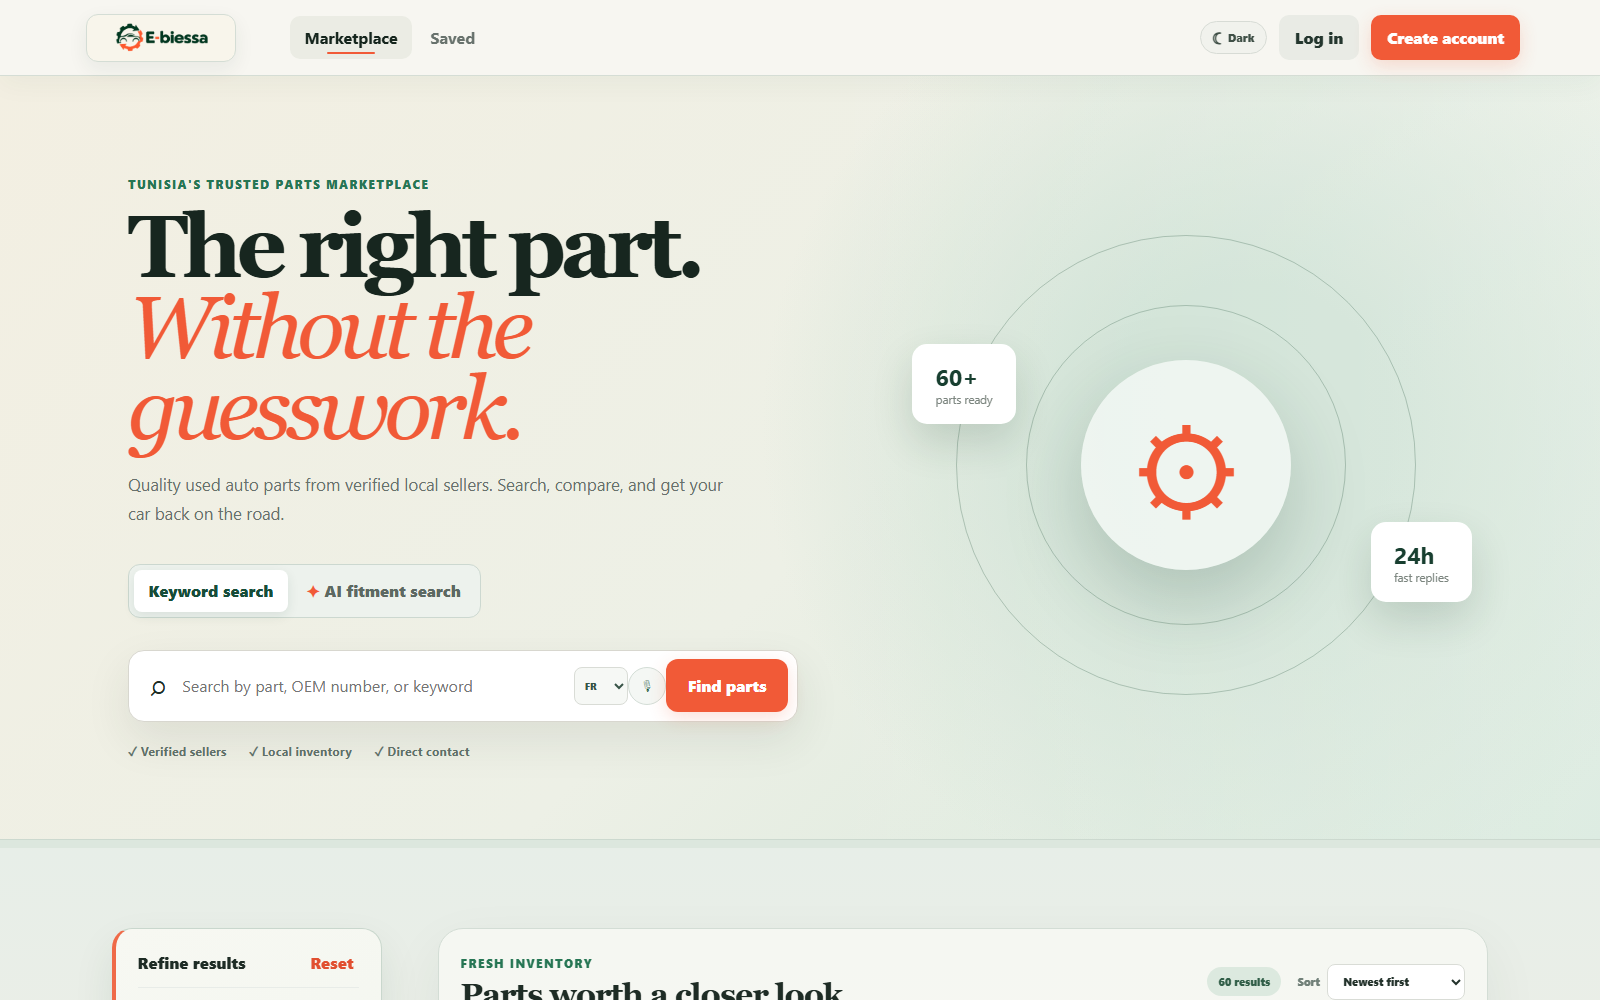
\includegraphics[width=\textwidth]{ui-marketplace.png}
\caption{Page d'accueil et accès à la recherche du marketplace E-biessa.}
\label{fig:ui-marketplace}
\end{figure}

\begin{figure}[H]
\centering
  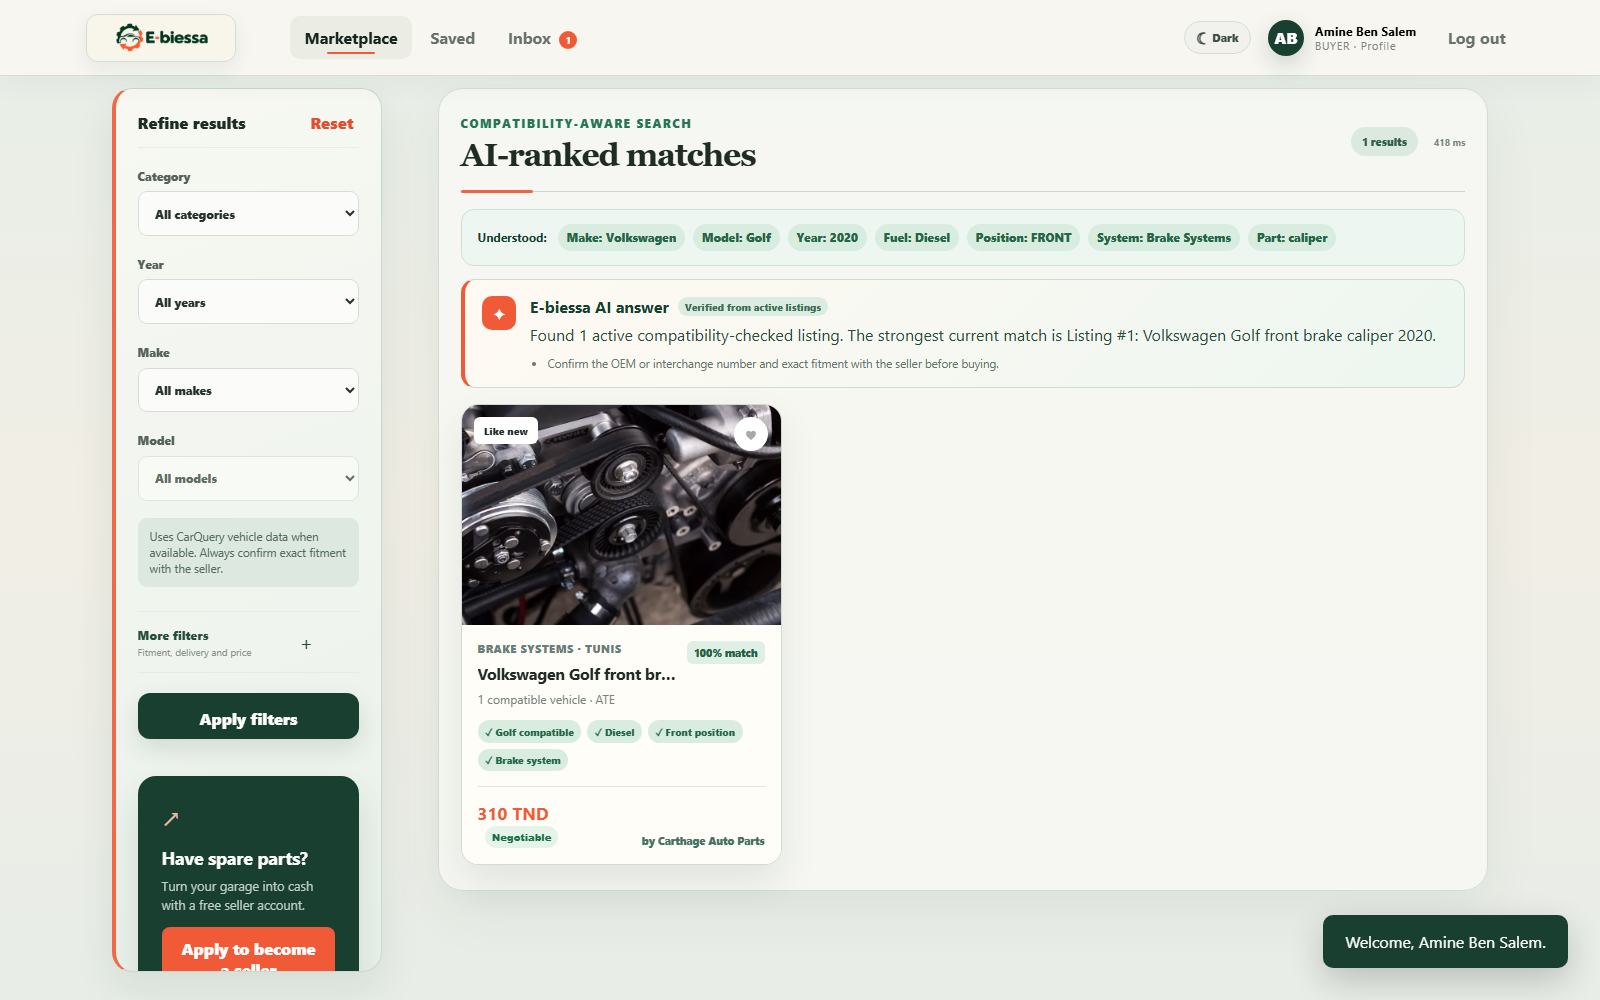
\includegraphics[width=\textwidth]{ui-ai-search.png}
\caption{Recherche IA avec contraintes extraites, réponse déterministe et explications de compatibilité.}
\label{fig:ui-ai-search}
\end{figure}

\begin{figure}[H]
\centering
  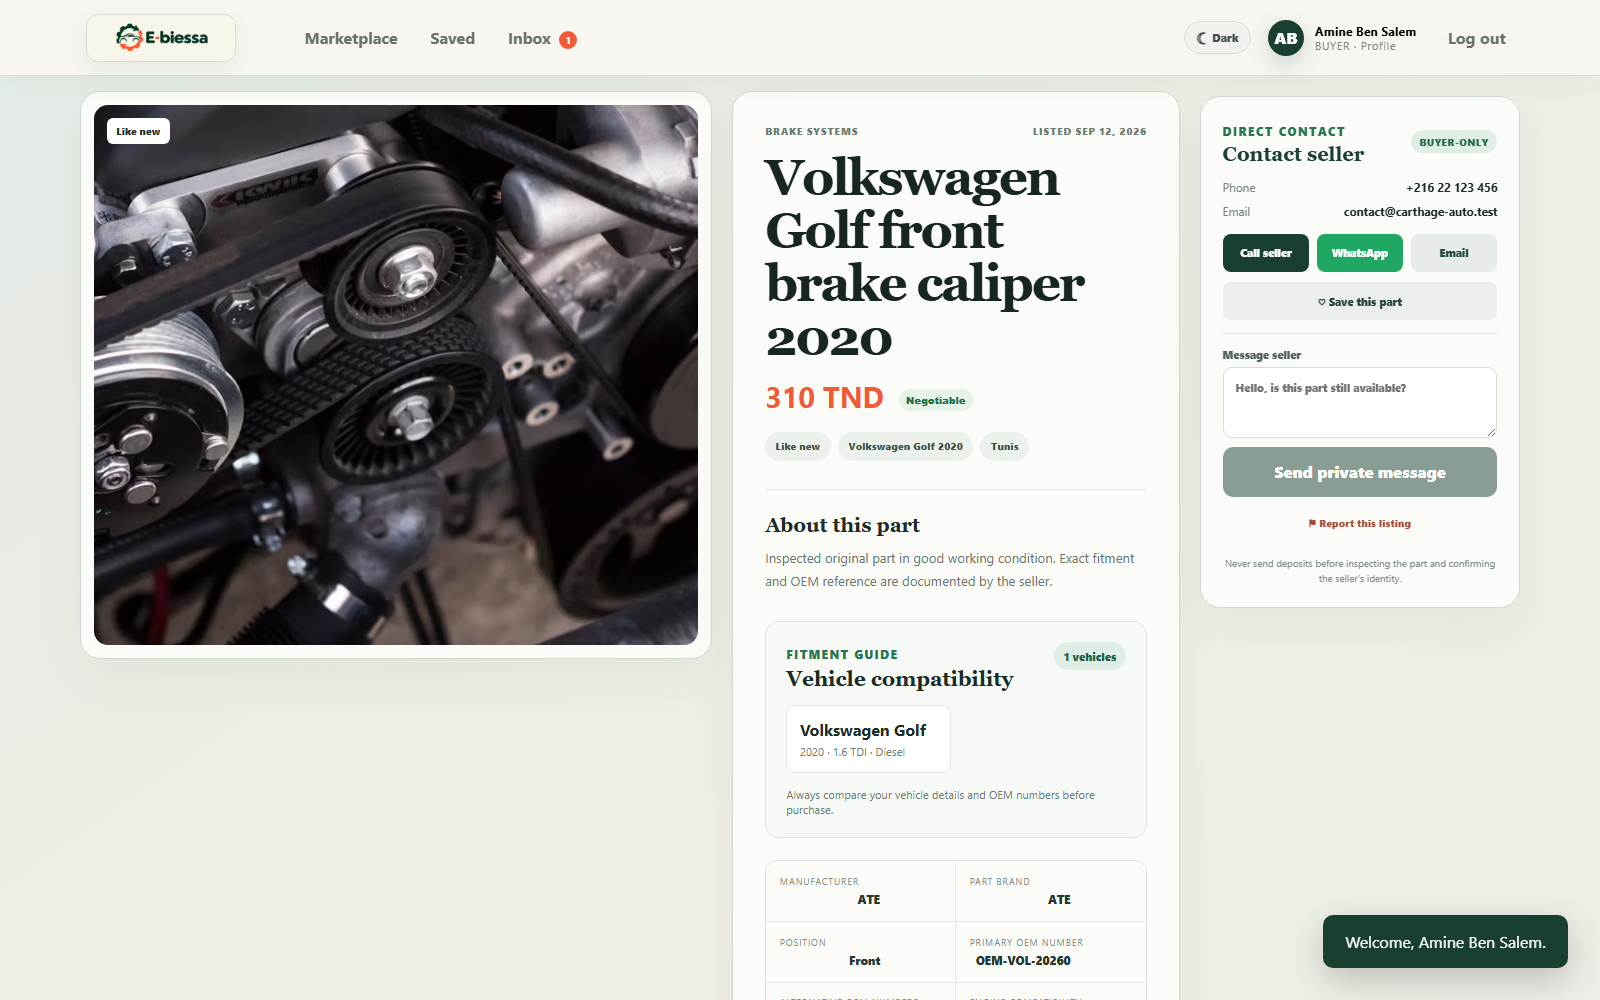
\includegraphics[width=\textwidth]{ui-listing-detail.png}
\caption{Fiche détaillée d'une pièce : compatibilité véhicule et contact vendeur protégé.}
\label{fig:ui-listing-detail}
\end{figure}

\begin{figure}[H]
\centering
  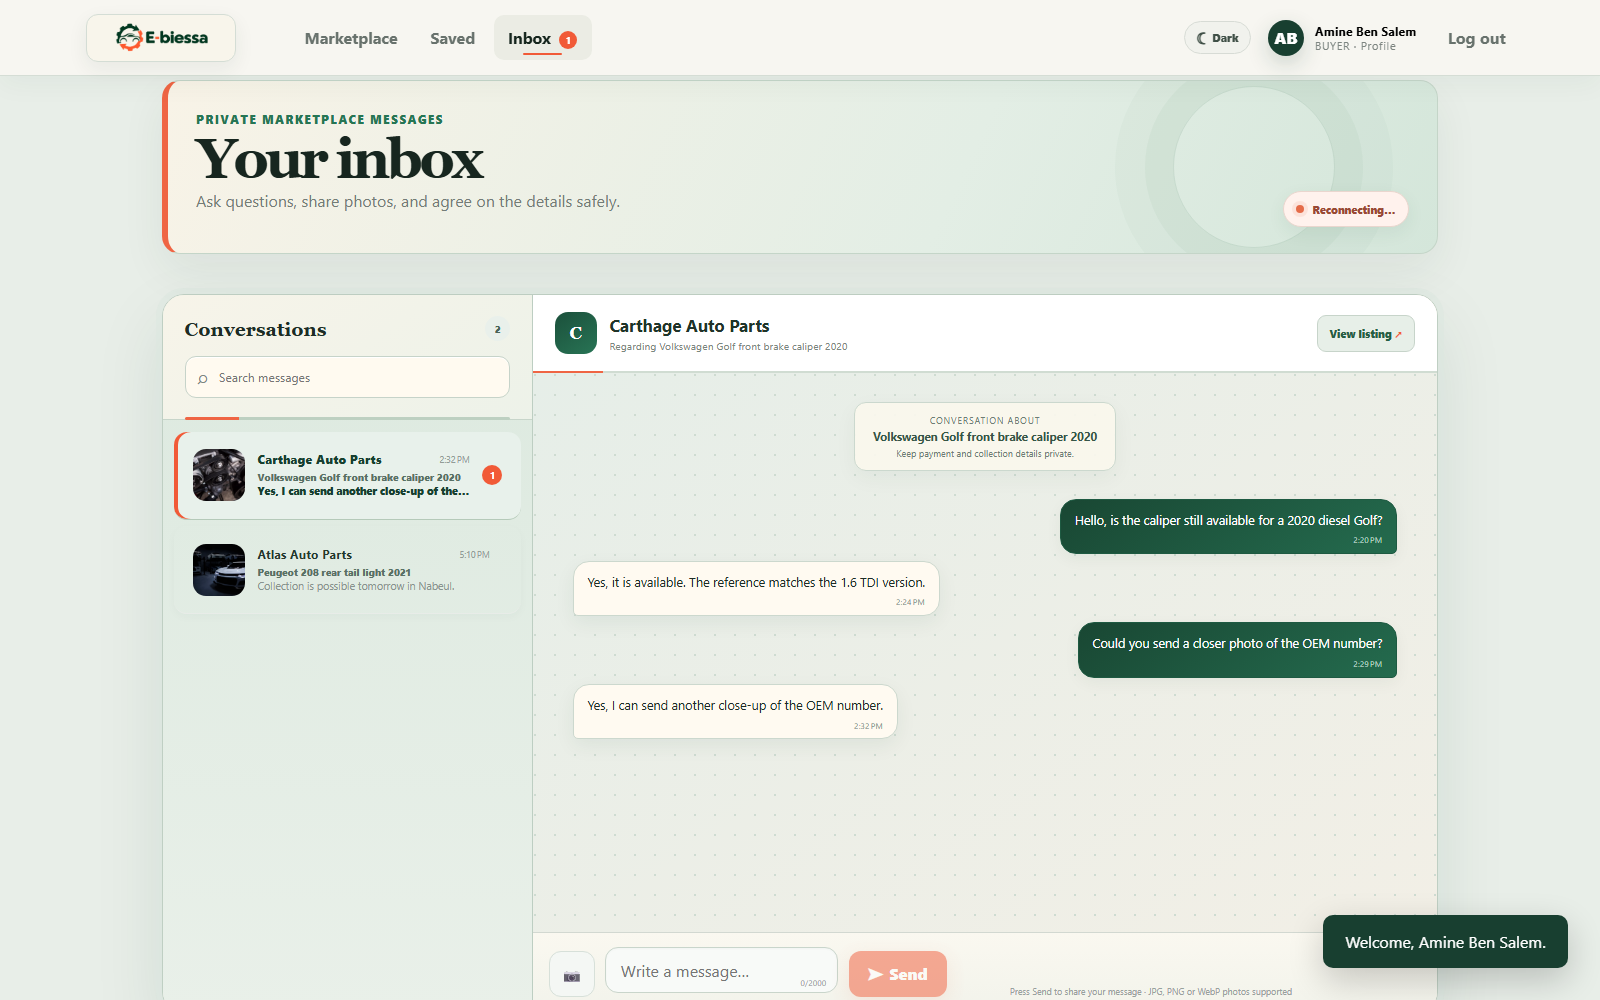
\includegraphics[width=\textwidth]{ui-messaging.png}
\caption{Boîte de réception et conversation privée entre acheteur et vendeur.}
\label{fig:ui-messaging}
\end{figure}

\begin{figure}[H]
\centering
  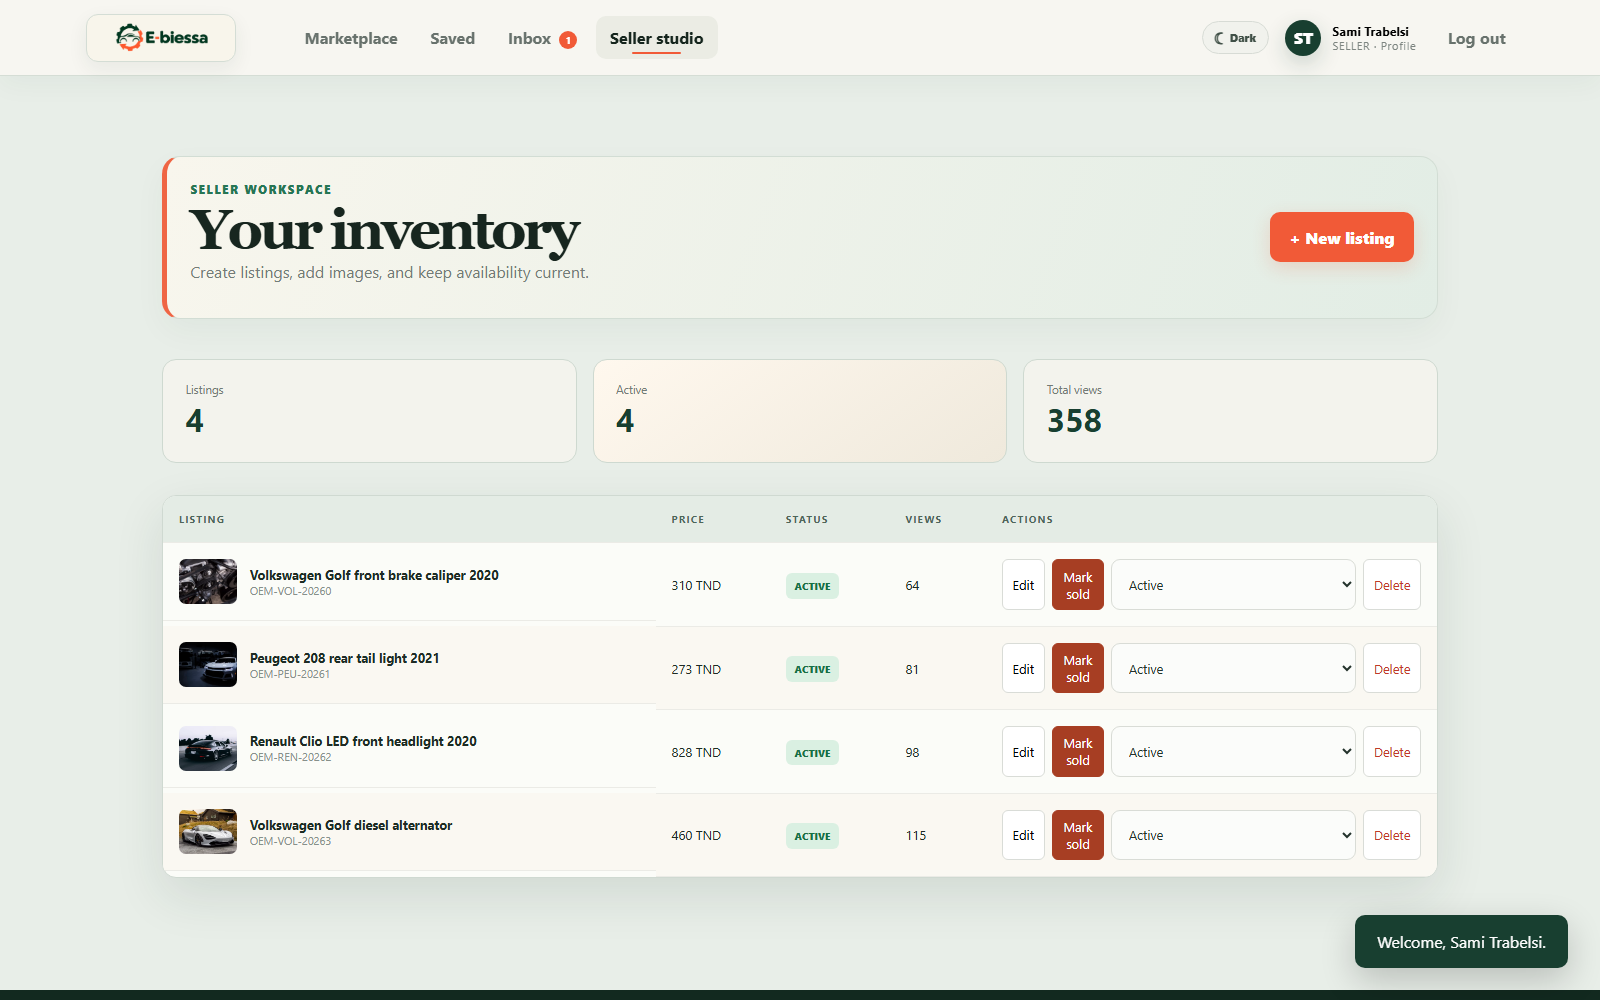
\includegraphics[width=\textwidth]{ui-seller-studio.png}
\caption{Studio vendeur pour le suivi des annonces, des statuts et des vues.}
\label{fig:ui-seller-studio}
\end{figure}

\begin{figure}[H]
\centering
  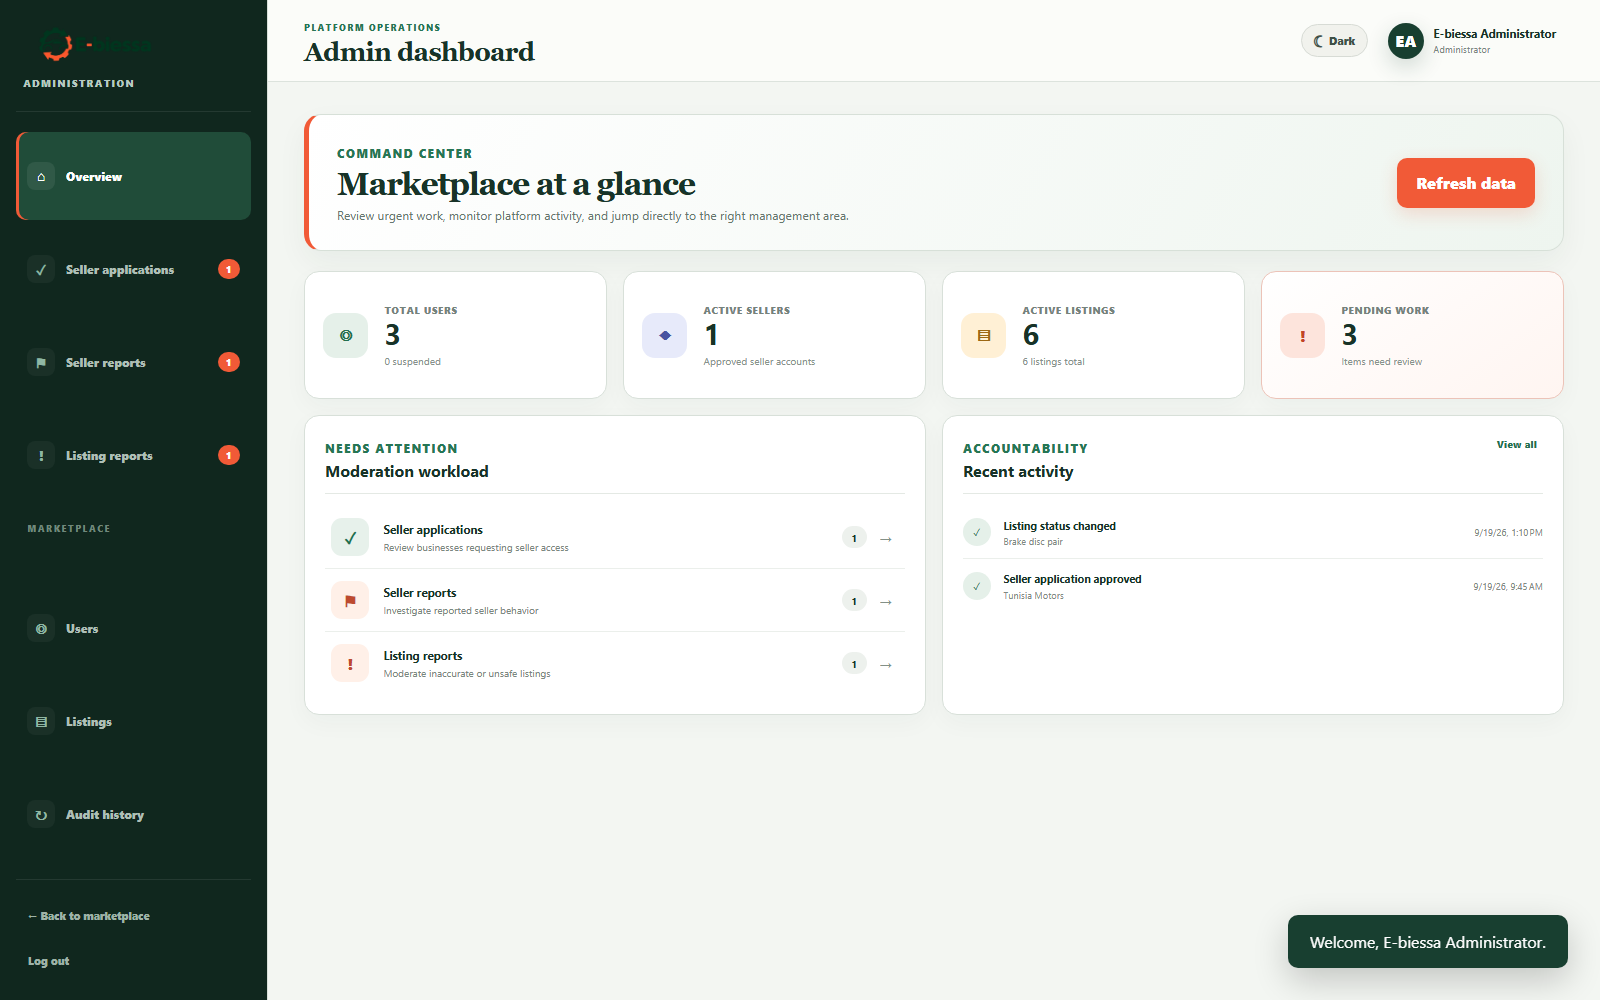
\includegraphics[width=\textwidth]{ui-admin-dashboard.png}
\caption{Tableau de bord administrateur et synthèse des files de modération.}
\label{fig:ui-admin-dashboard}
\end{figure}


\section{Gestion complète des annonces}

{\small\singlespacing\arrayrulecolor{tableline}
\begin{longtable}{|>{\raggedright\arraybackslash}p{\dimexpr 0.350\textwidth-2\tabcolsep-2\arrayrulewidth\relax}|>{\raggedright\arraybackslash}p{\dimexpr 0.650\textwidth-2\tabcolsep-2\arrayrulewidth\relax}|}
\hline
\rowcolor{tablehead} \color{white}\bfseries Bloc & \color{white}\bfseries Informations prises en charge \\ \hline
\endfirsthead
\rowcolor{tablehead} \color{white}\bfseries Bloc & \color{white}\bfseries Informations prises en charge \\ \hline
\endhead
\hline\endfoot
Identification & Titre, description, catégorie, fabricant, marque de pièce, OEM principal et alternatives \\ \hline
\rowcolor{tablerow} État commercial & Prix, négociable, état, garantie, livraison, collecte et localisation \\ \hline
Compatibilité & Plusieurs véhicules, année, moteur, carburant et position \\ \hline
\rowcolor{tablerow} Médias & JPEG/PNG/WebP, compression, ordre, image principale et suppression \\ \hline
Cycle de vie & Aperçu avant envoi ; états ACTIVE, INACTIVE, SOLD ; suppression séparée \\ \hline
\rowcolor{tablerow} Découverte & Filtres, tri, pagination, favoris, recherche IA et recommandations \\ \hline
\end{longtable}
}


\section{Comptes, profils et confiance}

L'identité locale est liée à l'adresse électronique et peut être complétée par Google, Facebook ou Microsoft lorsque les identifiants OAuth correspondants sont configurés. Le profil séparé contient nom, téléphone, localisation, nom commercial, site web et biographie. L'acheteur qui souhaite vendre soumet ces informations ; son statut reste en attente jusqu'à la décision d'un administrateur.


Un acheteur ayant déjà ouvert une conversation avec un vendeur peut lui attribuer de une à cinq étoiles et ajouter un commentaire facultatif. Un seul avis est conservé par couple acheteur--vendeur et peut être mis à jour. Cette condition atteste un contact, pas un achat confirmé : aucune commande payée n'est enregistrée dans la plateforme. La moyenne et le nombre d'avis sont publics. Les signalements et leur résolution administrative sont gérés séparément.


\section{Contact et messagerie}

La fiche annonce comporte une section « Contacter le vendeur ». Pour réduire l'extraction automatisée, les coordonnées ne sont renvoyées qu'à un acheteur connecté. Les boutons génèrent un appel téléphonique, un message WhatsApp préparé avec le titre de la pièce ou un courriel. L'acheteur peut aussi démarrer une conversation interne.


La boîte de réception présente une liste organisée de conversations et un panneau de discussion. Le fil possède une hauteur limitée, s'ouvre sur le dernier message et conserve le défilement vers les anciens échanges. L'envoi d'une image permet au vendeur de fournir des vues supplémentaires d'une pièce sans exposer un canal externe.


\section{Mise en oeuvre de l'IA}

Le modèle de base Qwen 2.5 7B Instruct a été chargé en 4 bits puis adapté avec Unsloth et LoRA de rang 8 sur un ordinateur équipé d'une RTX 4060 de 8 Go de VRAM et de 16 Go de mémoire système. Le jeu d'apprentissage contient des formulations anglaises, françaises et tunisiennes ainsi que les sorties JSON canoniques attendues. Une passe d'entraînement a été retenue après un test court, car les erreurs restantes concernaient surtout la copie de chiffres et relevaient mieux d'une validation déterministe que d'époques supplémentaires.


Le corpus corrigé v2 comprend 1 120 exemples d'apprentissage, 160 de validation et 120 de test. Les fichiers d'évaluation sont conservés séparément. La configuration locale limite la séquence à 256 tokens, utilise un lot de taille 1 et accumule les gradients sur huit étapes. Le taux d'apprentissage retenu pour l'époque v2 est de 0,00005.


Le modèle exporté est servi localement par Ollama sous le nom e-biessa-query-v2. FastAPI lui demande uniquement un objet structuré. La fonction de fusion contrôle ensuite l'année explicite, normalise les catégories et vérifie chaque valeur dans le catalogue. Cette approche apporte la souplesse linguistique du LLM tout en gardant un comportement reproductible.


\section{Jeu de démonstration}

Le profil de développement initialise un administrateur, trois acheteurs, trois vendeurs et soixante annonces réparties entre plusieurs marques, modèles, catégories et villes. Chaque vendeur possède plusieurs annonces détaillées. Les données sont réutilisables sans duplication au redémarrage et servent uniquement à la démonstration académique.


{\small\singlespacing\arrayrulecolor{tableline}
\begin{longtable}{|>{\raggedright\arraybackslash}p{\dimexpr 0.350\textwidth-2\tabcolsep-2\arrayrulewidth\relax}|>{\raggedright\arraybackslash}p{\dimexpr 0.650\textwidth-2\tabcolsep-2\arrayrulewidth\relax}|}
\hline
\rowcolor{tablehead} \color{white}\bfseries Donnée & \color{white}\bfseries Volume de démonstration \\ \hline
\endfirsthead
\rowcolor{tablehead} \color{white}\bfseries Donnée & \color{white}\bfseries Volume de démonstration \\ \hline
\endhead
\hline\endfoot
Administrateurs & 1 \\ \hline
\rowcolor{tablerow} Acheteurs & 3 \\ \hline
Vendeurs & 3 \\ \hline
\rowcolor{tablerow} Annonces actives initiales & 60 \\ \hline
Définitions véhicule locales & 20 \\ \hline
\rowcolor{tablerow} Langues d'exemple IA & anglais, français, arabe tunisien translittéré \\ \hline
\end{longtable}
}


\section{Configuration et exécution locale}

1. Démarrer MySQL et créer la base marketplace.


2. Définir les variables DB\_URL, DB\_USERNAME, DB\_PASSWORD, JWT\_SECRET et CORS\_ALLOWED\_ORIGINS dans l'environnement local de Spring.


3. Définir le même AI\_SERVICE\_TOKEN dans Spring et FastAPI, puis activer l'intégration IA.


4. Lancer Ollama avec le modèle adapté e-biessa-query-v2.


5. Démarrer FastAPI sur 127.0.0.1:8001, Spring Boot sur localhost:8080 et Angular sur localhost:4200.


6. Exécuter une réindexation complète avec le compte administrateur avant la première recherche sémantique.


\section{Assistance VIN et catalogue automobile}

Le profil acheteur propose la saisie d'un VIN de 17 caractères. Spring contrôle le format, interroge NHTSA vPIC puis rapproche la marque, le modèle, l'année et le carburant des lignes Vehicle du catalogue local. L'interface propose uniquement les identifiants locaux reconnus ; l'acheteur doit confirmer l'enregistrement de ses préférences. Une absence de correspondance conduit à la sélection manuelle, sans création automatique d'une compatibilité.


Le décodage utilise un délai configuré et un cache temporaire, fixé par défaut à 24 heures. Le VIN n'est pas persisté en base ; il est néanmoins transmis à NHTSA et intervient dans le cache de requête. La couverture vPIC, principalement orientée vers le marché américain, limite la reconnaissance de certains véhicules européens ou tunisiens. Le décodage n'est jamais présenté comme une garantie de montage.


\section{Estimation indicative du prix}

PriceEstimatorService compare la saisie du vendeur à un maximum de vingt annonces actives. Le score tient compte de la référence OEM, de la catégorie, des véhicules partagés, des termes du titre, de la position, de la marque de pièce et de l'état. L'annonce en cours d'édition et les vendeurs suspendus sont exclus. En l'absence de comparables suffisants, le système ne fabrique pas de prix.


La réponse fournit un prix central, une plage interquartile, le nombre de comparables et un niveau de confiance heuristique. Les quantiles de l'implémentation correspondent au rang arrondi dans la liste triée ; pour un effectif pair, le prix central n'est donc pas nécessairement la moyenne des deux valeurs centrales. Le calcul porte sur des prix demandés, pas sur des ventes conclues. Le vendeur conserve la décision et doit explicitement appliquer la suggestion.


\section{Identification de pièces par image}

L'utilisateur connecté peut transmettre une image JPEG, PNG ou WebP, limitée à 5 Mo. Spring applique l'authentification, la limitation de débit et les validations avant de transmettre les octets au service FastAPI avec le jeton interne. Le module optionnel utilise openai/clip-vit-base-patch32 pour comparer l'image à une taxonomie de vingt-deux types de pièces et retourner au plus cinq candidats.


Il s'agit d'une classification zero-shot, distincte de l'adaptation QLoRA de Qwen. Les scores sont relatifs aux catégories proposées, et non des probabilités calibrées de justesse. Le système ne déduit ni véhicule exact, ni référence OEM, ni garantie de compatibilité à partir des pixels. Le candidat choisi alimente une recherche dont les règles déterministes restent actives.


VISION\_ENABLED reste désactivé par défaut. L'activation requiert les dépendances de vision et le téléchargement initial du modèle, mis en cache pour les requêtes suivantes. Aucune fonction métier ne conserve la photo d'identification ni ne l'utilise pour l'apprentissage ; le traitement multipart peut toutefois recourir à des fichiers temporaires selon la configuration du serveur. Les tests automatisés isolent l'inférence au moyen d'un substitut.


\section{Saisie vocale}

Angular exploite la reconnaissance vocale proposée par le navigateur avec un choix français de Tunisie, arabe de Tunisie ou anglais américain. Le texte reconnu reste modifiable et la recherche ne part qu'après confirmation. L'absence de microphone, le refus de permission ou l'absence de prise en charge laisse disponible la saisie au clavier.


E-biessa reçoit la transcription, pas l'enregistrement audio. Le navigateur peut cependant faire appel au service vocal de son fournisseur ; la fonctionnalité ne doit pas être décrite comme une reconnaissance entièrement locale. Les tests utilisent un objet de reconnaissance simulé ; la qualité acoustique dépend d'une vérification réelle sur le navigateur et le microphone retenus.

\chapter{Tests et validation}

La validation combine des tests rapides par composant et des parcours représentatifs. Les chiffres présentés correspondent aux campagnes automatisées conservées avec le projet et à des jeux de données contrôlés.


\section{Stratégie}

La pyramide de tests couvre d'abord les règles métier isolées, puis les intégrations avec une base de test, les contrats du service IA et enfin les parcours dans un navigateur réel. Les scénarios sensibles - identité, propriété d'une annonce, compatibilité et visibilité des éléments vendus - sont testés à plusieurs niveaux.


{\small\singlespacing\arrayrulecolor{tableline}
\begin{longtable}{|>{\raggedright\arraybackslash}p{\dimexpr 0.240\textwidth-2\tabcolsep-2\arrayrulewidth\relax}|>{\raggedright\arraybackslash}p{\dimexpr 0.320\textwidth-2\tabcolsep-2\arrayrulewidth\relax}|>{\raggedright\arraybackslash}p{\dimexpr 0.440\textwidth-2\tabcolsep-2\arrayrulewidth\relax}|}
\hline
\rowcolor{tablehead} \color{white}\bfseries Niveau & \color{white}\bfseries Outil & \color{white}\bfseries Portée \\ \hline
\endfirsthead
\rowcolor{tablehead} \color{white}\bfseries Niveau & \color{white}\bfseries Outil & \color{white}\bfseries Portée \\ \hline
\endhead
\hline\endfoot
Backend & JUnit, Spring Boot Test, H2 & Services, contrôleurs, sécurité, sérialisation et persistance \\ \hline
\rowcolor{tablerow} Frontend & Vitest & Composants, formulaires, thèmes, erreurs et recommandations \\ \hline
IA & Pytest & Sécurité interne, normalisation, recherche et garde-fous \\ \hline
\rowcolor{tablerow} Navigateur & Playwright & Rôles, recherche IA, thèmes et parcours principaux \\ \hline
Modèle & Jeu de validation tenu à l'écart & JSON et exactitude par champ \\ \hline
\end{longtable}
}


\section{Résultats automatisés}

{\small\singlespacing\arrayrulecolor{tableline}
\begin{longtable}{|>{\raggedright\arraybackslash}p{\dimexpr 0.240\textwidth-2\tabcolsep-2\arrayrulewidth\relax}|>{\raggedright\arraybackslash}p{\dimexpr 0.320\textwidth-2\tabcolsep-2\arrayrulewidth\relax}|>{\raggedright\arraybackslash}p{\dimexpr 0.440\textwidth-2\tabcolsep-2\arrayrulewidth\relax}|}
\hline
\rowcolor{tablehead} \color{white}\bfseries Suite & \color{white}\bfseries Résultat validé & \color{white}\bfseries Observation \\ \hline
\endfirsthead
\rowcolor{tablehead} \color{white}\bfseries Suite & \color{white}\bfseries Résultat validé & \color{white}\bfseries Observation \\ \hline
\endhead
\hline\endfoot
Spring Boot & 62 tests réussis & Rapports JUnit locaux : sécurité, recommandations, VIN et prix \\ \hline
\rowcolor{tablerow} Angular & 51 tests réussis & Dernière campagne documentée ; image et voix incluses \\ \hline
FastAPI & 28 tests réussis & Dernière campagne documentée ; CLIP simulé dans les tests \\ \hline
\rowcolor{tablerow} Playwright isolé & 7 parcours réussis & Navigateur réel avec API contrôlée \\ \hline
Playwright pile complète & 4 scénarios opt-in non exécutés & Nécessite MySQL, Spring, FastAPI, Ollama et Angular actifs \\ \hline
\end{longtable}
}


\textbf{Lecture correcte des résultats}

Les tests Playwright isolés prouvent le comportement de l'interface dans un navigateur, mais ne remplacent pas une campagne sur la pile locale complète. Les deux suites sont donc conservées séparément.


Ces nombres décrivent les dernières campagnes consignées avant la revue documentaire, et non une nouvelle exécution de toutes les suites. Les rapports JUnit présents totalisent 62 tests sans échec. Les essais navigateur avec API simulée restent distincts des quatre scénarios de pile complète, désactivés par défaut. Ni ces comptes ni les simulations de CLIP et de microphone ne démontrent la précision de la vision ou de la reconnaissance vocale sur des données réelles.


\section{Évaluation du modèle de compréhension}

L'évaluation conservée dans training/v2-results-120.json porte sur 120 exemples tenus à l'écart de l'apprentissage. Elle mesure séparément la sortie brute de l'adaptateur et la chaîne corrigée. Un JSON syntaxiquement valide ne garantit pas la conformité du type de chaque champ, notamment celui de l'année.


{\small\singlespacing\arrayrulecolor{tableline}
\begin{longtable}{|>{\raggedright\arraybackslash}p{\dimexpr 0.350\textwidth-2\tabcolsep-2\arrayrulewidth\relax}|>{\raggedright\arraybackslash}p{\dimexpr 0.650\textwidth-2\tabcolsep-2\arrayrulewidth\relax}|}
\hline
\rowcolor{tablehead} \color{white}\bfseries Mesure & \color{white}\bfseries Résultat final \\ \hline
\endfirsthead
\rowcolor{tablehead} \color{white}\bfseries Mesure & \color{white}\bfseries Résultat final \\ \hline
\endhead
\hline\endfoot
JSON valide & 99,2 \% - 119/120 \\ \hline
\rowcolor{tablerow} Marque & 99,2 \% \\ \hline
Modèle & 96,7 \% \\ \hline
\rowcolor{tablerow} Carburant & 99,2 \% \\ \hline
Position & 99,2 \% \\ \hline
\rowcolor{tablerow} Catégorie canonique & 99,2 \% \\ \hline
\end{longtable}
}


Le type de pièce canonique atteint 99,2 \%. En revanche, l'année brute obtient 0 \% d'exactitude stricte et l'enregistrement brut complet obtient également 0 \%. Après validation autoritaire de l'année explicite, l'exactitude de l'enregistrement complet atteint 96,7 \% (116/120). Ce dernier chiffre caractérise donc la chaîne hybride, et non le modèle seul. Le petit jeu synthétique et les formes linguistiques qu'il couvre limitent toute généralisation à des utilisateurs réels.


\section{Validation de la recherche et des recommandations}

Le benchmark conservé dans training/retrieval-results.json comprend six requêtes synthétiques liées au catalogue de démonstration. HitRate@12, le rang réciproque moyen et l'exactitude des contraintes valent 1,0 sur ce jeu. Les six requêtes ne constituent ni une campagne statistique représentative ni une preuve d'efficacité en conditions réelles.


Les recommandations sont vérifiées sur le démarrage à froid, la correspondance exacte multi-véhicule, les carburants contradictoires, la priorité aux catégories sauvegardées, les vendeurs contactés, la diversité, les restrictions de rôle, l'effacement de l'historique et l'exclusion d'annonces supprimées. Les raisons retournées proviennent des mêmes signaux que le score.


\section{Recette fonctionnelle}

{\small\singlespacing\arrayrulecolor{tableline}
\begin{longtable}{|>{\raggedright\arraybackslash}p{\dimexpr 0.350\textwidth-2\tabcolsep-2\arrayrulewidth\relax}|>{\raggedright\arraybackslash}p{\dimexpr 0.650\textwidth-2\tabcolsep-2\arrayrulewidth\relax}|}
\hline
\rowcolor{tablehead} \color{white}\bfseries Scénario & \color{white}\bfseries Résultat attendu \\ \hline
\endfirsthead
\rowcolor{tablehead} \color{white}\bfseries Scénario & \color{white}\bfseries Résultat attendu \\ \hline
\endhead
\hline\endfoot
Acheteur recherche un étrier avant pour Golf diesel 2020 & Contraintes reconnues, aucune pièce arrière affichée \\ \hline
\rowcolor{tablerow} Vendeur marque une annonce vendue & Masquage immédiat des résultats publics ; synchronisation de l'index après transaction \\ \hline
Acheteur ouvre les coordonnées & Accès accordé uniquement avec le rôle Acheteur actif \\ \hline
\rowcolor{tablerow} Acheteur joint une photo à un message & Fichier validé, stocké et diffusé aux deux participants \\ \hline
Acheteur demande à devenir vendeur & Statut en attente jusqu'à décision administrateur \\ \hline
\rowcolor{tablerow} Administrateur suspend un vendeur & Connexion bloquée, annonces masquées et action auditée \\ \hline
Acheteur désactive la personnalisation & Historique comportemental supprimé, préférences explicites conservées \\ \hline
\rowcolor{tablerow} Index Qdrant contient un ID obsolète & Spring l'écarte lors du rechargement MySQL \\ \hline
\end{longtable}
}


\section{Limites et mesures compensatoires}

{\small\singlespacing\arrayrulecolor{tableline}
\begin{longtable}{|>{\raggedright\arraybackslash}p{\dimexpr 0.350\textwidth-2\tabcolsep-2\arrayrulewidth\relax}|>{\raggedright\arraybackslash}p{\dimexpr 0.650\textwidth-2\tabcolsep-2\arrayrulewidth\relax}|}
\hline
\rowcolor{tablehead} \color{white}\bfseries Limite & \color{white}\bfseries Mesure intégrée \\ \hline
\endfirsthead
\rowcolor{tablehead} \color{white}\bfseries Limite & \color{white}\bfseries Mesure intégrée \\ \hline
\endhead
\hline\endfoot
Catalogue CarQuery parfois indisponible & Repli local et confirmation explicite de la compatibilité par le vendeur \\ \hline
\rowcolor{tablerow} Petit jeu d'évaluation IA & Résultats présentés comme techniques, sans généralisation abusive \\ \hline
Données de démonstration & Comptes fictifs limités à la démonstration ; renouvellement avant diffusion \\ \hline
\rowcolor{tablerow} LLM sujet aux erreurs & Sortie structurée, normalisation, seuil et règles déterministes \\ \hline
Classement personnalisé content-based & Explications, désactivation, effacement et préparation à des évaluations humaines \\ \hline
\rowcolor{tablerow} Exécution académique locale & Architecture documentée et configuration externe pour une future mise en ligne \\ \hline
\end{longtable}
}


\section{Couverture du cahier des charges}

{\small\singlespacing\arrayrulecolor{tableline}
\begin{longtable}{|>{\raggedright\arraybackslash}p{\dimexpr 0.350\textwidth-2\tabcolsep-2\arrayrulewidth\relax}|>{\raggedright\arraybackslash}p{\dimexpr 0.650\textwidth-2\tabcolsep-2\arrayrulewidth\relax}|}
\hline
\rowcolor{tablehead} \color{white}\bfseries Périmètre & \color{white}\bfseries Réalisation et portée \\ \hline
\endfirsthead
\rowcolor{tablehead} \color{white}\bfseries Périmètre & \color{white}\bfseries Réalisation et portée \\ \hline
\endhead
\hline\endfoot
Phase 1 marketplace & Comptes, annonces, filtres, images, contact et administration ; transactions hors plateforme. \\ \hline
\rowcolor{tablerow} Phase 2 intelligence artificielle & Embeddings, Qdrant, extraction Qwen adaptée et réponses déterministes vérifiées. \\ \hline
Phase 3 orchestration & Outils LangChain en lecture seule, routage déterministe et recommandations explicables. \\ \hline
\rowcolor{tablerow} Extensions proposées & VIN, prix indicatif, identification CLIP optionnelle et saisie vocale. \\ \hline
Choix d'architecture & Spring Boot conservé pour le métier ; FastAPI consacré à l'IA, contrairement à un backend entièrement Python. \\ \hline
\rowcolor{tablerow} Limites de validation & Pas d'étude utilisateur représentative ; vision, voix et pile complète à qualifier sur les services réels. \\ \hline
Hors périmètre académique & Déploiement public, paiement, commandes, catalogue OEM certifié et garantie de compatibilité. \\ \hline
\end{longtable}
}


Le projet est achevé comme démonstrateur académique intégrant ces fonctions. La disponibilité des fournisseurs OAuth, du courriel, du SMS, de Cloudinary et de CLIP dépend des paramètres et des services activés. Le déploiement public, les migrations de schéma versionnées, la montée en charge et une étude utilisateur demeurent des travaux distincts ; ils ne sont pas présentés comme déjà validés.

\chapter*{Conclusion générale}
\addcontentsline{toc}{chapter}{Conclusion générale}

Le projet E-biessa aboutit à une plateforme complète de mise en relation autour des pièces automobiles d'occasion. Le socle transactionnel prend en charge les comptes, les rôles, les profils, les annonces riches, les images, la compatibilité multi-véhicule, les favoris, le contact, la messagerie, la réputation et l'administration. L'expérience Angular rend ces fonctions accessibles dans une interface cohérente et responsive.


L'apport majeur est l'intégration contrôlée de l'intelligence artificielle. Le modèle adapté comprend des formulations multilingues proches du langage des utilisateurs. La recherche vectorielle améliore le rappel, tandis que la validation déterministe protège la précision. Les recommandations et les agents spécialisés utilisent les mêmes principes : lecture seule, données minimales, raisons visibles et retour systématique à la source de vérité.


Ce travail a permis de mobiliser la conception orientée domaine, la sécurité web, les architectures distribuées, l'UX, le traitement du langage et l'évaluation expérimentale. La séparation Spring Boot / FastAPI représente un compromis justifié entre robustesse métier et agilité IA.


\section{Perspectives}

\begin{itemize}
\item déployer la pile derrière HTTPS après rotation et gestion centralisée des secrets ;

\item faire valider la compatibilité par des professionnels et intégrer des catalogues OEM sous licence ;

\item constituer un benchmark plus large, annoté manuellement, couvrant dialectes et fautes d'orthographe ;

\item mesurer la qualité des recommandations avec des retours anonymisés et des métriques hors ligne ;

\item ajouter notifications, paiement ou réservation uniquement après validation juridique et opérationnelle ;

\item surveiller dérive du modèle, qualité des données et taux de signalement avant tout usage public.
\end{itemize}

\chapter*{Bibliographie et webographie}
\addcontentsline{toc}{chapter}{Bibliographie et webographie}

[1] Spring, Spring Boot Reference Documentation, \url{https://docs.spring.io/spring-boot/}


[2] Spring, Spring Security Reference, \url{https://docs.spring.io/spring-security/reference/}


[3] Angular, Angular Documentation, \url{https://angular.dev/}


[4] FastAPI, FastAPI Documentation, \url{https://fastapi.tiangolo.com/}


[5] Qdrant, Qdrant Documentation, \url{https://qdrant.tech/documentation/}


[6] Ollama, Ollama Documentation, \url{https://docs.ollama.com/}


[7] Qwen Team, Qwen2.5 Technical Report, \url{https://arxiv.org/abs/2412.15115}


[8] Unsloth AI, Unsloth Documentation, \url{https://docs.unsloth.ai/}


[9] LangChain, LangChain Documentation, \url{https://docs.langchain.com/}


[10] OWASP Foundation, OWASP Top 10, \url{https://owasp.org/www-project-top-ten/}


[11] IETF, RFC 7519 - JSON Web Token, \url{https://www.rfc-editor.org/rfc/rfc7519}


[12] CarQuery API, Vehicle Data API, \url{https://www.carqueryapi.com/}


[13] Cloudinary, Image and Video API Documentation, \url{https://cloudinary.com/documentation/}


[14] Microsoft, Playwright Documentation, \url{https://playwright.dev/}

\appendix

\chapter{Cartographie des API}

{\small\singlespacing\arrayrulecolor{tableline}
\begin{longtable}{|>{\raggedright\arraybackslash}p{\dimexpr 0.350\textwidth-2\tabcolsep-2\arrayrulewidth\relax}|>{\raggedright\arraybackslash}p{\dimexpr 0.650\textwidth-2\tabcolsep-2\arrayrulewidth\relax}|}
\hline
\rowcolor{tablehead} \color{white}\bfseries Domaine & \color{white}\bfseries Exemples d'opérations \\ \hline
\endfirsthead
\rowcolor{tablehead} \color{white}\bfseries Domaine & \color{white}\bfseries Exemples d'opérations \\ \hline
\endhead
\hline\endfoot
Authentification & register, login, OAuth exchange, recovery request/complete \\ \hline
\rowcolor{tablerow} Annonces & list, detail, create, update, status, delete, my-listings \\ \hline
Images & upload, primary, order, delete \\ \hline
\rowcolor{tablerow} Vendeurs & profile, listings, contact, reviews, reports \\ \hline
Messagerie & inbox, start, detail, send text/image, realtime ticket \\ \hline
\rowcolor{tablerow} Recommandations & feed, settings, update settings, clear history \\ \hline
IA & semantic search, full reindex \\ \hline
\rowcolor{tablerow} Administration & users, seller applications, reports, moderation, audit \\ \hline
\end{longtable}
}

\chapter{Variables de configuration}

{\small\singlespacing\arrayrulecolor{tableline}
\begin{longtable}{|>{\raggedright\arraybackslash}p{\dimexpr 0.350\textwidth-2\tabcolsep-2\arrayrulewidth\relax}|>{\raggedright\arraybackslash}p{\dimexpr 0.650\textwidth-2\tabcolsep-2\arrayrulewidth\relax}|}
\hline
\rowcolor{tablehead} \color{white}\bfseries Variable & \color{white}\bfseries Usage \\ \hline
\endfirsthead
\rowcolor{tablehead} \color{white}\bfseries Variable & \color{white}\bfseries Usage \\ \hline
\endhead
\hline\endfoot
DB\_URL / DB\_USERNAME / DB\_PASSWORD & Connexion MySQL \\ \hline
\rowcolor{tablerow} JWT\_SECRET & Signature des jetons d'accès \\ \hline
CORS\_ALLOWED\_ORIGINS & Origines frontend autorisées \\ \hline
\rowcolor{tablerow} AI\_SERVICE\_TOKEN & Authentification interne Spring/FastAPI \\ \hline
AI\_SERVICE\_ENABLED & Activation de la recherche sémantique \\ \hline
\rowcolor{tablerow} OLLAMA\_BASE\_URL / OLLAMA\_MODEL & Accès au modèle local \\ \hline
CLOUDINARY\_* & Stockage distant optionnel des images \\ \hline
\rowcolor{tablerow} GOOGLE\_* / FACEBOOK\_* / MICROSOFT\_* & Fournisseurs OAuth optionnels \\ \hline
SMTP\_* / TWILIO\_* & Récupération de compte hors profil de développement \\ \hline
\end{longtable}
}


\textbf{Règle de gestion}

Les fichiers .env, les uploads, les index Qdrant, les caches, les modèles GGUF, les adaptateurs LoRA et les résultats Playwright sont exclus du dépôt Git.

\chapter{Commandes de validation}

Backend


cd marketplace-api
.\textbackslash{}mvnw.cmd test


Frontend


cd marketplace-frontend
npm run verify


Service IA


cd ai-service
.\textbackslash{}.venv\textbackslash{}Scripts\textbackslash{}python.exe -m pytest


E2E isolé


cd marketplace-frontend
npm run test:e2e


E2E pile complète


cd marketplace-frontend
npm run test:e2e:live

\chapter{Compléments techniques}

{\small\singlespacing\arrayrulecolor{tableline}
\begin{longtable}{|>{\raggedright\arraybackslash}p{\dimexpr 0.350\textwidth-2\tabcolsep-2\arrayrulewidth\relax}|>{\raggedright\arraybackslash}p{\dimexpr 0.650\textwidth-2\tabcolsep-2\arrayrulewidth\relax}|}
\hline
\rowcolor{tablehead} \color{white}\bfseries Fonction & \color{white}\bfseries Contrat ou paramètre \\ \hline
\endfirsthead
\rowcolor{tablehead} \color{white}\bfseries Fonction & \color{white}\bfseries Contrat ou paramètre \\ \hline
\endhead
\hline\endfoot
Décodage VIN & GET /api/vehicles/vin/\{vin\} ; authentification ; VIN\_DECODER\_ENABLED. \\ \hline
\rowcolor{tablerow} Prix indicatif & POST /api/parts/price-estimate ; vendeur ou administrateur. \\ \hline
Identification & POST /api/ai/identify ; fichier authentifié ; relais POST /v1/vision/identify. \\ \hline
\rowcolor{tablerow} Activation vision & VISION\_ENABLED ; requirements-vision.txt ; modèle CLIP mis en cache. \\ \hline
Personnalisation & GET /api/recommendations ; GET/PUT /api/recommendations/settings ; DELETE /api/recommendations/history. \\ \hline
\end{longtable}
}


La traçabilité technique s'appuie sur PROJECT\_HANDOFF.md, ARCHITECTURE.md, RECOMMENDATIONS.md, AGENT\_ORCHESTRATION.md, VIN\_COMPATIBILITY.md et IMAGE\_AND\_VOICE\_SEARCH.md. Les classes figurées proviennent du paquet entity du backend. Les métriques du modèle et de récupération proviennent respectivement de training/v2-results-120.json et training/retrieval-results.json.

\end{document}
